\documentclass[floatsintext,man]{apa6}

\usepackage{amssymb,amsmath}
\usepackage{ifxetex,ifluatex}
\usepackage{fixltx2e} % provides \textsubscript
\ifnum 0\ifxetex 1\fi\ifluatex 1\fi=0 % if pdftex
  \usepackage[T1]{fontenc}
  \usepackage[utf8]{inputenc}
\else % if luatex or xelatex
  \ifxetex
    \usepackage{mathspec}
    \usepackage{xltxtra,xunicode}
  \else
    \usepackage{fontspec}
  \fi
  \defaultfontfeatures{Mapping=tex-text,Scale=MatchLowercase}
  \newcommand{\euro}{€}
\fi
% use upquote if available, for straight quotes in verbatim environments
\IfFileExists{upquote.sty}{\usepackage{upquote}}{}
% use microtype if available
\IfFileExists{microtype.sty}{\usepackage{microtype}}{}

% Table formatting
\usepackage{longtable, booktabs}
\usepackage{lscape}
% \usepackage[counterclockwise]{rotating}   % Landscape page setup for large tables
\usepackage{multirow}		% Table styling
\usepackage{tabularx}		% Control Column width
\usepackage[flushleft]{threeparttable}	% Allows for three part tables with a specified notes section
\usepackage{threeparttablex}            % Lets threeparttable work with longtable

% Create new environments so endfloat can handle them
% \newenvironment{ltable}
%   {\begin{landscape}\begin{center}\begin{threeparttable}}
%   {\end{threeparttable}\end{center}\end{landscape}}

\newenvironment{lltable}
  {\begin{landscape}\begin{center}\begin{ThreePartTable}}
  {\end{ThreePartTable}\end{center}\end{landscape}}




% The following enables adjusting longtable caption width to table width
% Solution found at http://golatex.de/longtable-mit-caption-so-breit-wie-die-tabelle-t15767.html
\makeatletter
\newcommand\LastLTentrywidth{1em}
\newlength\longtablewidth
\setlength{\longtablewidth}{1in}
\newcommand\getlongtablewidth{%
 \begingroup
  \ifcsname LT@\roman{LT@tables}\endcsname
  \global\longtablewidth=0pt
  \renewcommand\LT@entry[2]{\global\advance\longtablewidth by ##2\relax\gdef\LastLTentrywidth{##2}}%
  \@nameuse{LT@\roman{LT@tables}}%
  \fi
\endgroup}


  \usepackage{graphicx}
  \makeatletter
  \def\maxwidth{\ifdim\Gin@nat@width>\linewidth\linewidth\else\Gin@nat@width\fi}
  \def\maxheight{\ifdim\Gin@nat@height>\textheight\textheight\else\Gin@nat@height\fi}
  \makeatother
  % Scale images if necessary, so that they will not overflow the page
  % margins by default, and it is still possible to overwrite the defaults
  % using explicit options in \includegraphics[width, height, ...]{}
  \setkeys{Gin}{width=\maxwidth,height=\maxheight,keepaspectratio}
\ifxetex
  \usepackage[setpagesize=false, % page size defined by xetex
              unicode=false, % unicode breaks when used with xetex
              xetex]{hyperref}
\else
  \usepackage[unicode=true]{hyperref}
\fi
\hypersetup{breaklinks=true,
            pdfauthor={},
            pdftitle={Measuring Adults' and Children's Comprehension of Disjunction},
            colorlinks=true,
            citecolor=blue,
            urlcolor=blue,
            linkcolor=black,
            pdfborder={0 0 0}}
\urlstyle{same}  % don't use monospace font for urls

\setlength{\parindent}{0pt}
%\setlength{\parskip}{0pt plus 0pt minus 0pt}

\setlength{\emergencystretch}{3em}  % prevent overfull lines


% Manuscript styling
\captionsetup{font=singlespacing,justification=justified}
\usepackage{csquotes}
\usepackage{upgreek}

 % Line numbering
  \usepackage{lineno}
  \linenumbers


\usepackage{tikz} % Variable definition to generate author note

% fix for \tightlist problem in pandoc 1.14
\providecommand{\tightlist}{%
  \setlength{\itemsep}{0pt}\setlength{\parskip}{0pt}}

% Essential manuscript parts
  \title{Measuring Adults' and Children's Comprehension of Disjunction}

  \shorttitle{Measuring Comprehension of Disjunction}


  \author{Masoud Jasbi\textsuperscript{1}~\& Michael C. Frank\textsuperscript{2}}

  % \def\affdep{{"", ""}}%
  % \def\affcity{{"", ""}}%

  \affiliation{
    \vspace{0.5cm}
          \textsuperscript{1} Harvard University\\
          \textsuperscript{2} Stanford University  }

  \authornote{
    All the experimental materials, data, randomization code, and analysis
    code for the studies reported in this paper are available in the
    following online repository:
    \url{https://github.com/jasbi/disjunction_comprehension}. The repository
    also includes instructions for reproducing this research.
    
    Correspondence concerning this article should be addressed to Masoud
    Jasbi, Boylston Hall, Cambridge, MA. E-mail:
    \href{mailto:masoud_jasbi@fas.harvard.edu}{\nolinkurl{masoud\_jasbi@fas.harvard.edu}}
  }


  \abstract{Disjunction has been a central topic in the literature on children's
semantic development. Previous research suggests that adults and
children might differ in their interpretation of linguistic disjunction
in two ways. First, unlike adults, children might interpret a
disjunction as conjunction (Singh, Wexler, Astle-Rahim, Kamawar, \& Fox,
2016; Tieu et al., 2016). Second, children might interpret \emph{or} as
inclusive disjunction when adults interpret it as exclusive (Crain,
2012). We first review the long tradition of research on children's
development of disjunciton. We argue that previous research suggests
conjunctive readings of disjunction are mainly due to task demands. Then
we present three studies that assess adults and children's understanding
of \emph{and} and \emph{or} using three different measures: binary truth
value judgments, ternary truth value judgments, and free-form verbal
feedback. We report that children and adults do not differ in their
binary judgments of disjunction. With ternary judgments, they show
similar results except when both disjuncts are true. Adults tend to rate
such disjunctions lower (exclusivity implicatures) while children
consider them ``right''. In their free-form verbal feedback, however,
children explicitly correct such infelicitous disjunctions and suggest
that the connective \emph{and} should have been used instead of
\emph{or}. These results suggest that forced-choice truth-value
judgments may underestimate children's pragmatic competence. In order to
capture children's semantic as well as pragmatic competence, we
recommend complementing truth value judgment tasks with measures more
sensitive to pragmatic infelicities.

Issues of measurement. Implications for pragmatic development.}
  \keywords{conjunction, disjunction, implicatures, semantics, pragmatics, logical
connectives, language, acquisition, development, children \\

    \indent Word count: X
  }





\usepackage{amsthm}
\newtheorem{theorem}{Theorem}
\newtheorem{lemma}{Lemma}
\theoremstyle{definition}
\newtheorem{definition}{Definition}
\newtheorem{corollary}{Corollary}
\newtheorem{proposition}{Proposition}
\theoremstyle{definition}
\newtheorem{example}{Example}
\theoremstyle{definition}
\newtheorem{exercise}{Exercise}
\theoremstyle{remark}
\newtheorem*{remark}{Remark}
\newtheorem*{solution}{Solution}
\begin{document}

\maketitle

\setcounter{secnumdepth}{0}



\subsection{Introduction}\label{introduction}

Disjunction has had a key role in advancing theories of logic, language,
and cognition. When introducing disjunction to students of logic, Alfred
Tarski (1941) complained about the complex factors that affect its
comprehension in everyday language:

\begin{quote}
\enquote{the usage of the word \emph{or} in everyday English is
influenced by certain factors of a psychological character. Usually we
affirm a disjunction of two sentences only if we believe that one of
them is true but wonder which one. If, for example, we look upon a lawn
in normal light, it will not enter our mind to say that the lawn is
green or blue, since we are able to affirm something simpler, and at the
same time, stronger, namely that the lawn is green. Sometimes even, we
take the utterance of a disjunction as an admission by the speaker that
he does not know which of the members of the disjunction is true.}
\end{quote}

In addition to the \textsc{speaker ignorance} effect of \emph{or},
Tarski noted that a disjunction has at least two different
interpretations. For example, a child may ask us to be taken to a hike
in the morning and a theater in the afternoon, but we may respond:
\enquote{No, we are going on a hike or we are going to the theater}. He
explained that disjunction in this example is \textsc{exclusive} because
\enquote{we intend to comply with only one of the two requests} and not
both. However, a disjunction may also have an \textsc{inclusive}
interpretation like the following example: \enquote{Customers who are
teachers or college students are entitled to a special reduction}.
Tarski explained that \emph{or} in this example is inclusive
\enquote{since it is not intended to refuse reduction to a teacher who
is at the same time a college student.} Tarski explained that there are
\enquote{quite noticeable differences between the usage of
{[}disjunction{]} in everyday language and in logic} and that
\enquote{the creators of contemporary logic, when introducing the word
\emph{or} into their considerations, desired, perhaps unconsciously, to
simplify its meaning and to render the latter {[}logical disjunction{]}
clear and independent of psychological factors.} Some logicians and
philosophers of language like P.F Strawson went even further and
suggested that \enquote{ordinary language has no exact logic} (Strawson,
1950).

The idea that there are noticeable differences between logical and
linguistic connectives remained common wisdom until H. Paul Grice's
\enquote{logic and conversation} (Grice, 1975). He contended that the
perceived differences between the meaning of natural language
connectives such as \emph{or} and the semantics of logical operators
such as \(\vee\) (inclusive disjunction) \enquote{arise from inadequate
attention to the nature and importance of the conditions governing
conversation.} He argued for two types of meaning: \enquote{what is
said} and \enquote{what is (conversationally) implied}. \enquote{What is
said} refers to the literal meanings of words; the conventional
association between words and meanings that is (relatively)
context-independent. \enquote{What is (conversationally) implied} (i.e.
\textsc{conversational implicature}), refers to meaning that is created
by using words and sentences in context. He contended that conversation
is governed by (at least) four maxims: be truthful (Maxim of Quality),
be informative (Maxim of Quantity), be relevant (Maxim of Relevance),
and be concise (Maxim of Manner). Conversational implicatures are
refinements to the literal meanings of words to make sure that the
utterance abides by the conversational maxims. As such, implicatures are
rational inferences and derived via the interaction of literal meaning
with conversational principles. In linguistics, the distinction between
\enquote{what is said} and \enquote{what is implied} gave rise to two
interrelated subfields in the study of meaning: semantics and
pragmatics.

Grice's main test case for his theory of meaning was the word \emph{or}.
He argued that the literal meaning of \emph{or} (i.e.~its semantics) is
inclusive disjunction as defined in classical logic. However, this
literal meaning is enriched in context to generate ignorance and
exclusivity inferences. Grice generalized and systematized Tarski's
intuition that we do not say \enquote{the lawn is green or blue} because
we can say \enquote{something simpler} (abiding by the Maxim of Manner),
and at the same time, stronger (abiding by the Maxim of Quantity): that
\enquote{the lawn is green}. Therefore, a disjunctive assertion commonly
results in the inference that the speaker could not have uttered only
one of the disjuncts, because s/he is uncertain about their truth
(ignorance inference). Similarly, exclusivity of a disjunction is
inferred by reasoning about the speaker's choice of the connective
(\emph{or} instead of \emph{and}). Going back to Tarski's example, the
child can reason that her dad could have said \enquote{we are going on a
hike \emph{and} we are going to the theater} if he intended to do both.
He used \emph{or} instead. Assuming he knows whether he wants to do both
or not, his utterance must mean means he wants to do one or the other
(exclusivity inference). Within the Gricean framework, ignorance and
exclusivity of \emph{or} are secondary inferences, derived from the
interaction of its literal (inclusive) meaning with conversational
principles. Grice's arguments gave rise to a radical methodological and
theoretical shift in the study of meaning in philosophy and linguistics.

In psychology, disjunction and its related words such as the English
\emph{or} have played an important role in advancing theories of logical
thought and its development in humans (Inhelder \& Piaget, 1958; Neisser
\& Weene, 1962). Early studies tested adults and children's
comprehension of logical words such as \emph{and}, \emph{or}, and
\emph{not} as a proxy for human logical understanding (Neimark, 1970;
Neimark \& Slotnick, 1970; Nitta \& Nagano, 1966). Influenced by the
arguments that language has no logic, researchers asked at what age
logical (inclusive) and nonlogical (exclusive) understanding of
disjunction develops. They arrived at the conclusion that while the
logical meaning of conjunction and negation were understood early, the
logical meaning of disjunction was a late development; in fact as late
as highschool or college years. Advances and improvements in the methods
used to test adults and children's linguistic comprehension convinced
some researchers that the logical understanding of disjunction is
present in school years, but not in preschool (Braine \& Rumain, 1981).

The advent of the Gricean approach to meaning shifted the research
question, from the development of logical and nonlogical concepts, to
the development of the semantics and pragmatics of logical words. Some
developmental researchers argued that by advancing methods that separate
semantic from pragmatic competence in children, they show an early
understanding for the truth conditions of linguistic connective
\emph{or} as inclusive disjunction (Chierchia, Crain, Guasti, \&
Thornton, 1998; chierchia2004semantic; Crain, 2012). According to Crain
(2012), not only children's understanding of disjunction matches its
semantics in classical logic, but it is also probable that this
understanding is part of an innate logical endowment (Crain \&
Khlentzos, 2008, 2010). Since the start of research on children's
development of disjunction, more than 30 research papers have been
published on the topic and this number is sure to increase as research
on disjunction sheds light on various aspects of human understanding and
development of meaning and logic.

The research presented here builds on this long and well-established
literature in two ways. First, it further improves on previous
experimental methods. Some previous experimental studies used complex
experimental design, complex linguistic stimuli, or alternatively lacked
appropriate controls such as a control connective or comprehension of
adults in the same task. In section \ref{litreview} we review these
issues and in section \ref{study1} we present an experimental paradigm
that avoids them. Second, most previous research tested children and
adults using two-alternative forced-choice tasks (2AFC) (Crain \&
Thornton, 1998). Here, we report adults and children's judgments with
both two and three alternatives (2AFC and 3AFC tasks). We also compare
children's truth value judgments against their open-ended verbal
feedback to the speaker.

Study 1 (section \ref{study1}) tested adults' interpretations of
connectives \emph{and} and \emph{or} in the context of a guessing game
using 2AFC and 3AFC truth value judgment tasks. The 2AFC task showed
that adults interpret \emph{and} as conjunction and \emph{or} as
inclusive disjunction in the guessing game. The 2AFC task did not show
sensitivity to the pragmatics of disjunction in the game. The 3AFC task,
however, showed sensitivity to the pragmatics of disjunction:
participants were more likely to pick the middle option among three
alternatives, when both disjuncts were true. Comparing the 2AFC and 3AFC
results, the 2AFC task underestimated judgments of felicity and better
approximated truth judgments compared to the 3AFC task. This finding is
intuitive given that more options provide a better opportunity to
express nuances of linguistic interpretation.

Study 2 (section \ref{study2}) investigated preschool children's
judgments in the same guessing game as study 1 using a 3AFC task. We
used three alternatives to give children a better chance of expressing
their pragmatic knowledge and judgments of felicity (Katsos \& Bishop,
2011). The study also analyzed and categorized children's open-ended
verbal feedback in the task. Both the 3AFC judgments and the categories
of open-ended responses showed that four-year-olds differentiated
\emph{or} from \emph{and}. While children's judgments in the 3AFC task
showed no sign of infelicity for disjunctive guesses when both disjuncts
were true, their open-ended feedback showed that children find such
guesses infelicitous. In their open-ended feedback, children explicitly
emphasized the word \emph{and} as what the speaker (i.e.~puppet) should
have used instead of \emph{or}, when both disjuncts were true.

Study 3 (section \ref{study3}) used the same paradigm as study 2, but
focused on replicating preschool children's open-ended responses and
contrasting them with the results of a 2AFC task. As in study 2, both
truth judgments and open-ended feedback showed that children
differentiated \emph{or} from \emph{and}. The 2AFC task showed no
evidence that children find disjunctions with true disjuncts
infelicitous. However, children's judgments did not differ significantly
from those of adults in the 2AFC task of study 1. As in study 2,
children's open-ended feedback suggested that when both disjuncts were
true, children found a disjunctive statement infelicitous and the
conjunctive alternative more appropriate. Overall, the results of study
2 and 3 show that forced-choice judgement tasks underestimate children's
pragmatic competence. In contrast, systematic analysis of children's
open ended verbal feedback captured children's sensitivity to pragmatic
violations. We conclude that using open-ended elicitation and analysis
of children's feedback \textbf{together with} forced choice truth
judgment tasks may provide us with better measurements of children's
true semantic and pragmatic competence.

\subsection{Previous Research}\label{litreview}

Research on children's comprehension of logical connectives \emph{and}
and \emph{or} consists of two periods. The first period (1960s-80s) was
inspired by Piaget's developmental theory (Inhelder \& Piaget, 1958).
Researchers in this period sought to discover the development of basic
logical concepts such as negation, conjunction, and disjunction.
Following Inhelder and Piaget (1958), they predicted that children first
form concrete concepts for conjunction and disjunction between the ages
of 7-11 years (concrete operational stage) and only after 11 (formal
operational stage) do they develop an abstract and logical understanding
of these words. While later research in this period rejected this
timeline, it upheld the claim that a logical (inclusive) understanding
of disjunction develops late. The second period (since late 90s) is
inspired by Grice's theory of meaning, specifically his distinction
between semantics and pragmatics. Researchers in this period argued that
previous studies conflated semantic and pragmatic knowledge and used
methods that vastly underestimated children' semantic competence. By
controlling for the role of pragmatics and focusing on children's truth
judgments, they aimed to show that children have early and adult-like
semantics for logical words such as \emph{or}. Based on these results,
they argued that the understanding of logical concepts and their role in
language is likely innate (Crain \& Khlentzos, 2008, 2010). In what
follows, we review the highlights of these two traditions and end with a
note on how the studies presented here contribute to this long-standing
research on development of disjunction.

To examine the Piagetian theory, Nitta and Nagano (1966) tested 679
Japanese students (grades K, 2, 4, 6, and 8) and Neimark and Slotnick
(1970) conducted a similar study on 455 English-speaking children in
grades 3-8 and 58 college students. Participants were tested on
negation, conjunction, and disjunction. Each question provided six
response options; for example a fish, a bird, and a flower, each with a
white and a black version. Participants were asked to \enquote{circle
all the items} described by statements such as: \enquote{flower},
\enquote{not bird}, \enquote{bird and flower}, \enquote{bird or flower},
\enquote{black and bird}, \enquote{black or flower}, etc. These studies
concluded that the majority of the participants understood negation and
conjunction, but only college students correctly answered statements
containing a disjunction. They reported that participants made two types
of errors. First across all ages, some participants interpreted
disjunction as conjunction. For example they circled black birds when
the instruction said \enquote{black or bird}. Second, some selected only
one of the two categories. Based on these results Neimark (1970)
concluded that a \enquote{correct} (i.e.~inclusive) understanding of
disjunction only develops in the high school years and depends on the
attainment of formal operations as defined in the Piagetian theory.

Paris (1973) used a similar in-classroom setup to test children's
comprehension of connectives in Grades 2, 5, 8, 11, and college. Two
hundred participants (40 per grade) were asked to judge the truth of
sentences with the connectives \emph{and}, \emph{or}, and
\emph{either-or}. The experimenter showed participants slides of
pictures, for example a bird in a nest, with descriptions such as
\enquote{the bird is in the nest or the shoe is on the foot.} The
participants were asked to judge the statement as true or false. Paris
found that statements with \emph{and} were almost always judged
correctly, but this was not the case with disjunction. First, he
reported that older participants produced more errors when both
disjuncts were true, presumably because they interpreted disjunctions as
exclusive and not inclusive. Second, the majority of younger children,
and even around a fifth of college students considered a disjunction
false when only one of the disjuncts was true. The combination of these
two trends suggested that younger children and even some adults did not
differentiate \emph{or} from \emph{and}, interpreting both as
conjunction. Finally, Paris also found that there were fewer errors with
\emph{either-or} statements compared to \emph{or} statements. He
suggested that the word \emph{either} could provide further cue on how
disjunction should be interpreted. Paris (1973) attributed the
conjunctive interpretations of \emph{or} to the application of
non-linguistic strategies when an utterance is hard to interpret (See
Clark, 1973 for a discussion of nonlinguistic strategies in child
language acquisition). He suggested that children in his task were
\enquote{comparing visual and auditory information with little regard
for the implied logical relationship in the verbal description.} In
other words, children responded with \enquote{true} if the individual
disjuncts matched the pictures and false otherwise. Such a
non-linguistic strategy would yield correct answers for conjunction but
incorrect (conjunctive) answers for disjunction. This explains why
conjunctive readings reduce with age and why using the word
\emph{either} helped reduce conjunctive interpretations further.

After Paris (1973), it was understood that the in-class tests were not
suitable for testing participants' linguistic competence and certainly
not suitable for younger children. Therefore, Johansson and Sjolin
(1975) set out to examine the interpretation of disjunction in a simpler
\enquote{Give-item} task. They tested preschool Swedish-speaking
children's comprehension of conjunction and disjunction in present tense
sentences (e.g. \enquote{Richard wants to drink lemonade or milk. Show
me what he drank!}) and imperative sentences (e.g. \enquote{Put up
{[}the picture of{]} the car or the doll!}). They reported that starting
(at least) at age four, children interpreted the Swedish equivalents of
\emph{and} and \emph{or} as conjunction and exclusive disjunction. They
argued that the linguistic \emph{or} should be kept separate from the
logical notion of (inclusive) disjunction. While linguistic
understanding of \emph{or} develops early as exclusive disjunction, the
logical understanding of it develops late.

Braine and Rumain (1981) is the only study that tested the same
participants with both a Give-item task and a version of what is today
known as the Truth Value Judgment Task. They tested 22 children in each
of the age groups 5-6, 7-8, and 9-10 years, as well as 22 adults. In the
Give-item task, 14 wooden blocks with varying shapes, colors, and sizes
were used (a replication of Suppes \& Feldman, 1969). Experimenters
asked participants the following: 1) \enquote{Give me all the green
things or give me all the round things} and 2) \enquote{Give me all
those things that are either blue or round.} They reported that for both
commands and in both children and adults, the most likely response was
to give all the objects that had only one of the properties. They
considered these results as evidence for a \enquote{choose-one}
(i.e.~exclusive) interpretation of disjunction in the context of
imperatives. In the judgment task, a puppet described the contents of
four boxes that each contained four animal toys. For example, the puppet
said \enquote{Either there is a horse or a duck in the box.} The first
box had both animals, the second had only a horse, the third only a
duck, and the last had neither. Participants were asked if the puppet
was right. The results showed that adults were split between an
inclusive and an exclusive interpretation of disjunction. The 7-8 and
9-10 year-olds were more likely to consider the disjunction as
inclusive. However, the youngest group (5-6 years old) was most likely
to interpret a disjunction similar to a conjunction: they said the
puppet was right when both animals were in the box and not right or
partly right if only one of the animals was in the box. Following Paris
(1973), Braine and Rumain (1981) argued that younger children do not
take the contribution of the connective \emph{or} into account. Instead,
they use a non-linguistic strategy in which the disjunction is right if
both propositions are true, partly right if only one is true, and wrong
if neither is true.

Braine and Rumain (1981) concluded that children's ability to interpret
a disjunction in a command develops earlier than their ability to judge
truth values. It is important to note that in Braine and Rumain (1981)'s
judgment task, the puppet used a disjunction even though the content of
the box was known to both the puppet and the participant (i.e.~it lacked
ignorance). As Tarski (1941) noted, such uses of disjunction sound odd
and infelicitous. More generally, a disjunction such as \enquote{A or B}
is infelicitous when discourse participants already know which
proposition is true. Later truth value judgment studies such as
Chierchia et al. (1998) controlled for this effect of disjunction by
making the puppet utter disjunction as a prediction of an unknown event,
and let participants judge the prediction after they see the outcome of
the event.

Chierchia et al. (1998) kicked off the second period of inquiry into
children's comprehension of disjunction. Following Grice (1989), they
differentiated between semantic knowledge, which includes the knowledge
of truth values, and pragmatic knowledge. They contended that
interpreting logical connectives involves a semantic and a pragmatic
component, and that the semantics of logical connectives cannot be
assessed if the role of pragmatics is not controlled for. More
specifically, they argued that felicitous use of a disjunction requires:
(i) a set of alternatives (ii) evidence that one of them holds (iiia)
evidence that not all of them hold, or (iiib) uncertainty as to whether
all of them hold. While the semantics of \emph{or} is inclusive, a
variety of factors including pragmatic reasoning can provide evidence
that not all alternatives hold. For example, we may reason that given
speaker's knowledge of the situation, they could have used the
connective \emph{and} if all alternatives were true. Therefore, to
understand the semantic contribution of disjunction, we should test
participants in contexts which are stripped from pragmatic factors that
contribute to exclusivity.

Chierchia et al. (1998) tested 23 English-speaking and 10
Italian-speaking children in two conditions: description mode and
prediction mode. In both conditions, a troll considered whether to eat a
hamburger, a piece of pizza, or an ice-cream and went ahead to eat a
piece of pizza and an ice-cream but not a hamburger. In description
mode, Kermit described what happened as \enquote{A troll ate a piece of
pizza or an ice cream} while in prediction mode, Kermit used the same
sentence as a prediction before the troll eats his lunch. They reported
that in the description mode, children accepted Kermit's statement when
both disjuncts were true less than one-third of the time. However, in
prediction mode, they accepted such sentences 100\% of the time. They
argued that when we control for the effect of pragmatics on
interpretation, children understand disjunction as inclusive, and
conform to the semantics of disjunction in classical logic.

Following Chierchia et al. (1998), several studies have argued that
preschool children's knowledge of disjunction conforms to the
predictions of classical logic and formal semantics in environments as
varied as negative sentences (Crain, Gualmini, \& Meroni, 2000),
conditional sentences (Gualmini, Crain, \& Meroni, 2000), restriction
and nuclear scope of the universal quantifier \emph{every} (Chierchia,
Crain, Guasti, Gualmini, \& Meroni, 2001; Chierchia et al., 2004),
nuclear scope of the negative quantifier \emph{none} (Gualmini \& Crain,
2002), restriction and nuclear scope of \emph{not every} (Notley,
Thornton, \& Crain, 2012), and prepositional phrases headed by
\emph{before} (Notley, Zhou, Jensen, \& Crain, 2012), as well as similar
environments in other languages such as Mandarin Chinese and Japanese
(Goro \& Akiba, 2004; Su, 2014; Su \& Crain, 2013). These studies also
commonly reported that in linguistic environments where adults consider
a disjunction exclusive, children are more likely to consider it
inclusive. Since under the Gricean account, exclusive interpretation of
disjunction is the result of pragmatic (scalar) implicatures, these
findings are considered as further evidence for the hypothesis that
young children do not compute implicatures at the rate that adults do
(Barner, Brooks, \& Bale, 2011; Noveck, 2001; Papafragou \& Musolino,
2003).

It is important to note that all the studies mentioned above in the
Gricean period use the Truth Value Judgment Task (Crain \& Thornton,
1998). As mentioned earlier, Braine and Rumain (1981) found that the
same children were more likely to interpret a disjunction as exclusive
in a give-item task and inclusive/conjunctive in a truth value judgment
task. Therefore, it is possible that truth value judgment tasks are
simply not suitable for capturing children' knowledge of exclusivity
implicatures. Furthermore, several studies listed above test children's
knowledge of disjunction in environments that largely collapse the
distinction between \emph{and} and \emph{or}. For example, in the
restriction of \emph{every}, a conjunction and a disjunction can result
in the same interpretation (e.g. \emph{Every man or woman is happy} vs.
\emph{Every man and woman is happy}). Therefore, successful
interpretation in these studies can also be achieved by applying the
nonlinguistic strategies that result in conjunctive interpretations, as
discussed by the early studies (Braine \& Rumain, 1981; Paris, 1973).

More recently, some studies have revived the earlier findings that
preschool children may interpret disjunction as conjunction. Singh et
al. (2016) tested 56 English-speaking children (M=4;11, 3;9-6;4) and 26
adults in a truth value judgment task. The experiment involved four
pictures: a boy holding a banana, a boy holding an apple and a banana,
three boys holding either an apple or a banana, and three boys holding
both apples and bananas. In each trial, participants saw one of the
pictures and a puppet described the pictures with four possible
utterances: \enquote{The/every boy is holding an apple or/and a banana.}
Participants were asked: \enquote{Was {[}the puppet{]} right or wrong
about this picture?} They found that children were more likely to say
the puppet was right when both disjuncts were true than when only one
was. They concluded that \enquote{many preschool children - the majority
in {[}the study's{]} sample - understand disjunctive sentences \ldots{}
as if they were conjunctions.} Tieu et al. (2016) also found evidence
for conjunctive interpretations of disjunction in preschool children.
They tested 28 French-speaking children (3;7-6;6, M=4;5) and 18
Japanese-speaking children (4;7-6;6, M=5;5) as well as 20
French-speaking and 21 Japanese-speaking adults. They used the
\enquote{prediction mode} of the Truth Value Judgment Task, in which the
puppet provides a prediction or guess, an event occurs, and participants
are asked if the prediction was right. For example, there was a chicken
on the screen, next to a toy bus and a toy plane. The puppet appeared on
the screen and predicted that \enquote{the chicken pushed the bus or the
plane.} Then the chicken pushed either one or both of the objects.
Participants stamped on a happy face or a sad face to show whether the
puppet's guess was right or wrong. Like Singh et al. (2016), they
reported that unlike adults, children were more likely to consider the
disjunctive guess right when both disjuncts were true, rather than only
one. They concluded that children - the majority of them in their sample
- interpreted disjunction as conjunction.

However, a recent replication of Tieu et al. (2016) by Skordos, Feiman,
Bale, and Barner (2018) suggests that the high rate of conjunctive
interpretations were most likely due to experimental design. They tested
126 preschoolers in three conditions: replication (N=43, 4;0-5;9,
M=5;0), modified script (N=41, 4;0-5;10, M=5;0), and three-alternatives
(N=42, 4;0-5;11, M=5;0). The first condition was a direct replication of
Tieu et al. (2016). The second, modified script, removed some
experimenter comments right after the puppet's guess that could
potentially confuse children. The comments were: \enquote{Look! The
chicken pushed that! She didn't want to break that one. So she didn't
touch it. So was {[}the puppet{]} right?} The third condition,
three-alternatives, was similar to modified-script but provided three
objects; for example a plane, a bus, and a bicycle. The reasoning was
that if there are only two alternatives, a disjunction is trivially
true, and consequently children may consider that unacceptable. The
results replicated Tieu et al. (2016)'s findings in the replication
condition, but showed that conjunctive interpretations of disjunction
disappeared almost completely in the third condition with three
alternatives. Skordos et al. (2018) concluded that children's
conjunctive interpretations are most likely due to non-linguistic
strategies applied when they are uncertain about some aspect of the
experimental task. This conclusion is similar to the conclusions of
Paris (1973) and Braine and Rumain (1981) in earlier studies.

To summarize, previous studies show that experimental tasks can have a
big impact on our conclusions regarding children's comprehension of
disjunction. Early in-class tasks suggested that even high-schoolers do
not interpret a disjunction correctly and confuse it with \emph{and}.
Improving on task design, Braine and Rumain (1981) argued that this is
only the case in preschool children. They also showed that the same
children can have different interpretations of disjunction in different
tasks: in a Give-item task they interpret it as exclusive while in a
truth value judgment task they interpret it as conjunctive or inclusive.
Using various versions of the truth value judgment task, research in the
Gricean tradition has argued that preschool children understand the
semantics of disjunction and interpret it as inclusive. However, this
line of research has also suggested that children are insensitive to the
exclusivity implicature of disjunction. While some recent studies have
argued that preschool children may interpret disjunction as conjunctive,
a replication study has argued that conjunctive interpretations were
largely due to task demands.

Here we improve on previous studies by first controlling for various
factors that had proven problematic before, and second investigating the
role of task measurement in assessing preschool children's
interpretation of disjunction. As explained above, previous research has
shown that in studying children's interpretation of disjunction, it is
important to control for the following factors:

\begin{enumerate}
\def\labelenumi{\arabic{enumi}.}
\tightlist
\item
  complexity of the linguistic stimuli,
\item
  complexity of the task,
\item
  ignorance of the speaker with respect to the truth of the disjuncts,
\item
  interpretation of the conjunction word (e.g. \emph{and}) in the same
  task
\item
  interpretation of adults in the same task.
\item
  discernibility of conjunctive and disjunctive interpretations in the
  task
\end{enumerate}

Some previous studies used complex linguistic stimuli or relatively
complex designs that may have increased the application of
non-linguistic strategies. Some studies violated \enquote{speaker
ignorance}; i.e.~had the speaker utter the disjunction when the truth of
the propositions were known to the speaker. Some studies did not use the
conjunction word (e.g. \emph{and}) in control trials, or did not use
adults as control participants. Finally, some studies tested the
disjunction word in linguistic environments that collapse interpretive
differences between a conjunction a disjunction. The experimental
paradigm reported here builds and improves on previous studies by
controlling for all these factors.

In the studies reported here, we used simple existential sentences (e.g.
\emph{there is a cat or a dog}) and tested the interpretation of
participants in a simple and easy to understand guessing game. The
guessing game provided a context in which the speaker was ignorant with
respect to to which alternatives were true. The game is essentially a
variant of the truth value judgment task and used conjunction trials as
well as adult participants as controls. Conjunction and disjunction
trials resulted in different interpretations in the task. Furthermore,
we tested children's interpretations in two different ways, using forced
choice tasks with 2 and 3 options (2AFC and 3AFC tasks), as well as
free-form verbal responses.

\subsection{Study 1: Adult's 2AFC and 3AFC Judgments}\label{study1}

The goal of this study was to examine adults' interpretations of
\emph{and} and \emph{or} as a benchmark for children's interpretations.
Participants saw a card, read a description, and had to evaluate the
description with respect to what they saw on the card. In test trials,
the descriptions contained the conjunction word \emph{and} and the
disjunction word \emph{or}. We tested adults in both two-alternative and
three-alternative forced choice tasks (2AFC and 3AFC). The results
suggested that adults interpreted \emph{and} as conjunction and
\emph{or} as inclusive disjunction. Adults also considered statements
with \emph{or} infelicitous when both disjuncts were true. The study
also found that the 2AFC and 3AFC tasks registered different aspects of
adult interpretations: the 2AFC task captured adult intuitions on the
basic semantics of the connectives while the 3AFC task was sensitive to
pragmatic infelicities as well.

\subsubsection{Methods}\label{methods}

\paragraph{Materials and Design}\label{materials-and-design}

\begin{figure}[!h]

{\centering 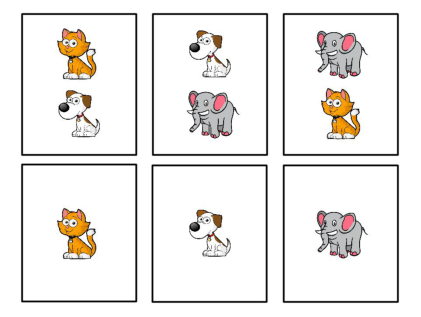
\includegraphics{figs/stimuli-1} 

}

\caption{Cards used in the connective guessing game.}\label{fig:stimuli}
\end{figure}

We used six cards with cartoon images of a cat, a dog, and an elephant
(Figure \ref{fig:stimuli}). There were two types of cards: cards with
only one animal and cards with two animals. There were three types of
guesses: simple (e.g. \emph{There is a cat}), conjunctive (e.g.
\emph{There is a cat and a dog}), and disjunctive (e.g. \emph{There is a
cat or a dog}). In each guess, the animal labels used in the guess and
the animal images on the card could have no overlap (e.g.~Image: dog,
Guess: \emph{There is a cat or an elephant}), partial overlap
(e.g.~Image: Cat, Guess: \emph{There is a cat or an elephant}), or total
overlap (e.g.~Image: cat and elephant, Guess: \emph{There is a cat or an
elephant}). Crossing the number of animals on the card, the types of
guesses, and the overlap between the guess and the card yields 12
different possible trial types. We chose 8 trial types (Figure
\ref{fig:trials}), to balance the number of one-animal vs.~two-animal
cards, simple vs.~connective guesses, and expected true vs.~false
trials.

\begin{figure}[!h]

{\centering 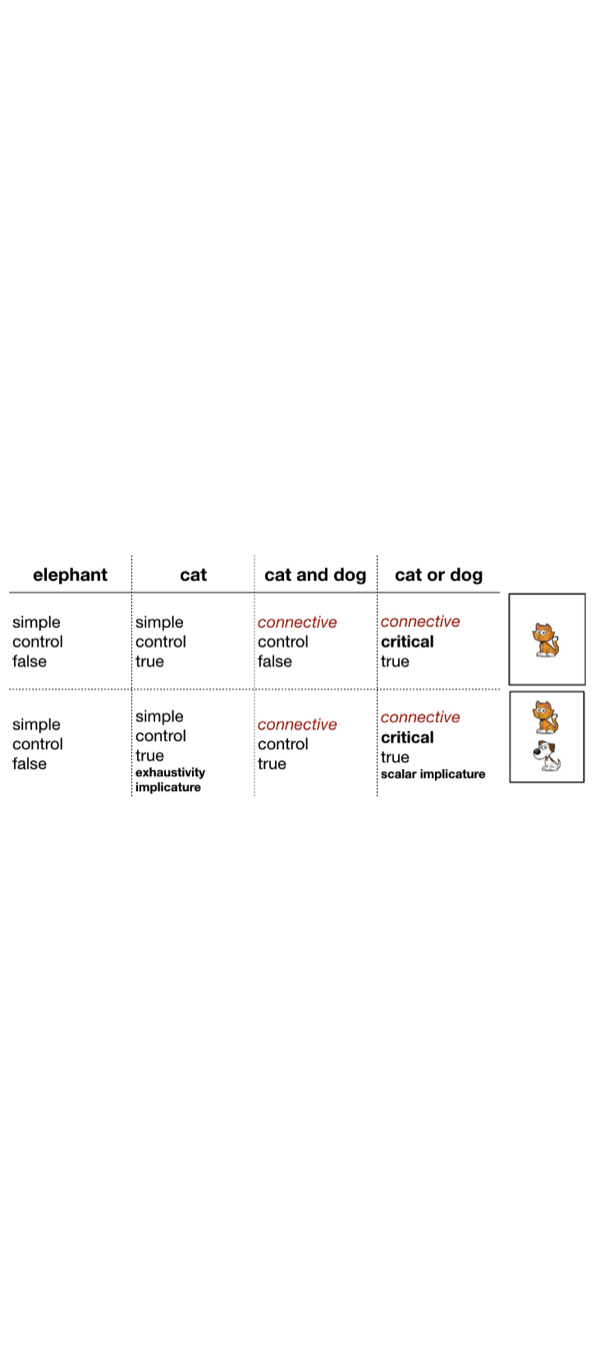
\includegraphics{figs/trials-1} 

}

\caption{Trial types represented by example cards and example guesses.}\label{fig:trials}
\end{figure}

\paragraph{Participants and Procedure}\label{participants-and-procedure}

\begin{figure}[!h]

{\centering 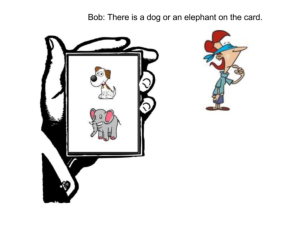
\includegraphics{figs/exampleTrial-1} 

}

\caption{An example trial in Study 1.}\label{fig:exampleTrial}
\end{figure}

We used Amazon's Mechanical Turk (MTurk) for recruitment and the online
platform Qualtrics for data collection and survey design. The task took
about 5 minutes on average to complete. 109 English speaking adults
participated. 57 of them were assigned to a 2AFC judgment task and 52 to
a 3AFC judgment task. In the 2AFC task, participants had to judge using
the options \enquote{wrong} and \enquote{right}. In the 3AFC task they
had to choose between \enquote{wrong}, \enquote{kinda right}, and
\enquote{right}. The two conditions were otherwise identical. There are
many possible labels for the middle option \enquote{kinda right},
including \enquote{kinda wrong} or \enquote{neither}. A later
experiment, tested different intermediate labels and found that adults
consider \enquote{kinda right} to be a more suitable option for
capturing pragmatic infelicities (see Jasbi, Waldon, \& Degen,
submitted). We expect similar behavior from labels like \enquote{a bit
right} and \enquote{a little right} which refer to non-maximal degrees
of being \enquote{right}.

The experiment had three phases: introduction, instruction, and test. In
the introduction, participants saw the six cards and read that they
would play a guessing game. Then a blindfolded cartoon character named
Bob appeared on the screen. Participants were told that in each round of
the game, they would see a card and Bob was going to guess what animal
was on the card. The study emphasized that Bob could not see anything.
Participants were asked to judge whether Bob's guess was right. In the
instruction phase, participants saw an example trial where a card with
the image of a dog was shown with the following sentence written above
Bob's head: \emph{There is a cat on the card}. All participants
correctly responded with \enquote{wrong} and proceeded to the test
phase.

In the test phase, participants saw one trial per trial type. Within
each trial type, the specific card-guess scenario was chosen at random.
The order of trial types was also randomized. At the end of the study,
participants received \$0.4 as compensation. Figure
\ref{fig:exampleTrial} shows an example test trial.

\begin{longtable}[]{@{}lllll@{}}
\caption{\label{tab:study1info}Summary of study 1 methods with adult
participants}\tabularnewline
\toprule
Study & N & Age & Mode & Response Options\tabularnewline
\midrule
\endfirsthead
\toprule
Study & N & Age & Mode & Response Options\tabularnewline
\midrule
\endhead
Study 1 - 2AFC & 57 & Adults & Online (Mturk) & Wrong,
Right\tabularnewline
Study 1 - 3AFC & 52 & Adults & Online (Mturk) & Wrong, Kinda Right,
Right\tabularnewline
\bottomrule
\end{longtable}

\subsubsection{Results}\label{results}

In this section, we first present the results of the 2AFC and 3AFC tasks
with adults. Then we discuss how these results can be interpreted with
respect to the semantics and pragmatics of disjunction in the context of
the guessing game.

\begin{figure}
\centering
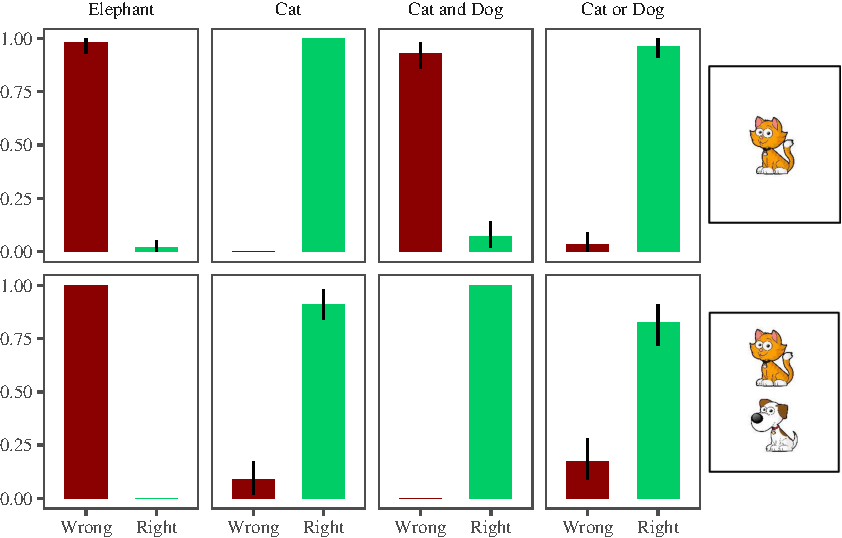
\includegraphics{figs/binaryAdultsPlot-1.pdf}
\caption{\label{fig:binaryAdultsPlot}Adults' two-alternative forced choice
judgments.}
\end{figure}

Figure \ref{fig:binaryAdultsPlot} shows the results for the adult 2AFC
task. The two left columns show the simple guesses and serve as
controls. The results show that if the animal mentioned in the guess was
not on the card (e.g., elephant), participants judged the guess to be
\enquote{wrong}; if the animal was on the card (e.g., cat), participants
judged the guess to be \enquote{right}. The next two columns of Figure
\ref{fig:binaryAdultsPlot} show the results for the test conditions,
namely conjunction and disjunction. An \emph{and}-guess (e.g.~cat and
dog) was considered \enquote{wrong} if only one of the animals was on
the card, and \enquote{right} if both were. An \emph{or}-guess (e.g.~cat
or dog) was \enquote{right} whether one or both animals were on the
card. The patterns of \enquote{right} and \enquote{wrong} responses in
the binary task match the expectations for truth and falsehood of
logical conjunction and (inclusive) disjunction.

\begin{figure}
\centering
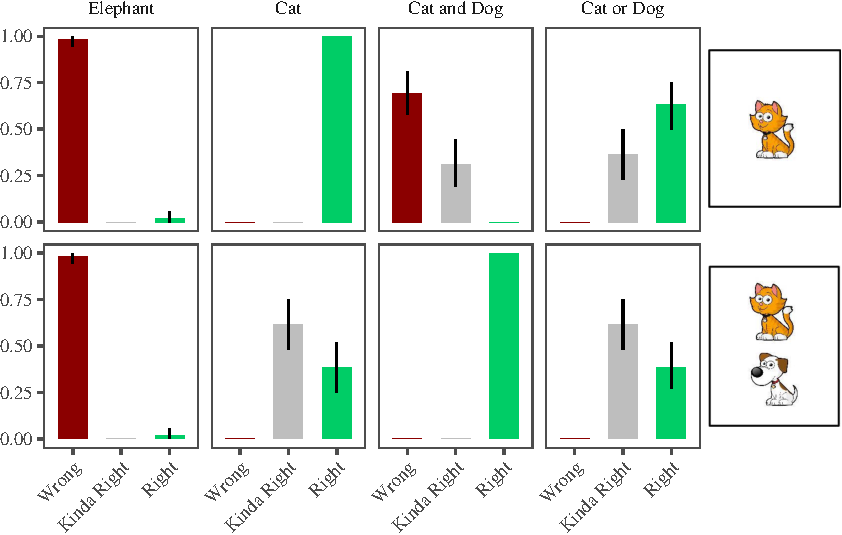
\includegraphics{figs/ternaryAdultsPlot-1.pdf}
\caption{\label{fig:ternaryAdultsPlot}Adults' three-alternative forced
choice judgments in the connective guessing game.}
\end{figure}

Figure \ref{fig:ternaryAdultsPlot} shows the results for the 3AFC
judgment task. For four trial types, the results were identical to the
2AFC task. In the first and second trial types, if the animal mentioned
was not on the card (e.g.~elephant), participants judged the guess as
\enquote{wrong}, regardless of whether one animal was on the card or
two. In the third trial type, if the animal mentioned (e.g.~cat) was the
only animal on the card, participants judged the guess as
\enquote{right}. Finally, if there were two animals on the card and the
puppet mentioned them using \emph{and} (e.g.~cat and dog), all
participants considered the guess \enquote{right}.

The four remaining trial types showed different patterns of judgments
than their counterparts in the 2AFC task. If the animal mentioned
(e.g.~cat) was only one of the animals on the card, participant
judgments were divided between \enquote{right} and \enquote{kinda
right}. When only one of the animals was on the card (e.g.~cat) and the
guess was a conjunction (e.g cat and dog), most adults considered the
guess \enquote{wrong} but some chose \enquote{kinda right}, perhaps
suggesting that the intermediate option was used to express that one of
the animals was correctly guessed. With disjunctive guesses (e.g.~cat or
dog), if the card had only one of the animals (e.g.~cat), most
participants considered the guess \enquote{right} while some considered
it \enquote{kinda right}. It is possible that those who chose
\enquote{kinda right} considered the right guess to be \enquote{cat}.
For disjunctive trials with both animals on the card, adults were split
between \enquote{kinda right} and \enquote{right} responses. The choice
of \enquote{kinda right} over \enquote{right} in such trials can be
interpreted as a sign that adults were sensitive to the infelicity of a
disjunction when conjunction was more appropriate. In the next section,
we discuss the nature of pragmatic reasoning in the context of this
guessing game.

\subsubsection{Discussion}\label{discussion}

Consider the following truth conditions for \emph{and} and \emph{or}: A
conjunction with \emph{and} is true when both conjuncts are true and
false otherwise. An inclusive disjunction with \emph{or} is true when at
least one disjunct is true and false otherwise. An exclusive disjunction
is true when only one of the disjuncts is true and false otherwise.
Let's also assume a simple linking function in which false statements
are judged as \enquote{wrong} and true statements as \enquote{right}
(see Jasbi et al. (submitted) for a discussion of linking assumptions in
this task). In the context of study 1, this purely truth-conditional
account has the following predictions: First, conjunctive guesses like
\enquote{cat and dog} are wrong when only one of the animals is on the
card and right when both are. Second, disjunctive guesses are always
right if they are interpreted as inclusive, because in all such trials
at least one of the animals is present on the card. However, if
disjunctive guesses are exclusive, they are right when one of the
animals is on the card and wrong when both are. Finally, the addition of
a third intermediate option between wrong and right should not
substantially affect the judgments.

Figure \ref{fig:binaryAdultsPlot} shows that in 2AFC judgments, the
predictions are borne out for \emph{and} as conjunction and \emph{or} as
inclusive disjunction, but not exclusive disjunction. The majority of
disjunctive guesses were considered right in the 2AFC task and in the
3AFC task, no disjunctive guess was judged wrong. These results suggest
that inclusive disjunction better captures the truth-conditions of
\emph{or} in the existential sentences of this paradigm. However, in the
3AFC task, judgments deviated from a purely truth-conditional account in
four trial types: (i) trials with simple guesses when two animals were
shown on the card; (ii) disjunction trials with one animal; (iii)
disjunction trials with two animals; and (iv) conjunction trials with
one animal on the card.

These trial types fall into two major categories with respect to their
response patterns. First, those in which participants chose
\enquote{kinda right} and \enquote{right} (i-iii); Second, those in
which participants chose \enquote{wrong} and \enquote{kinda right} (iv).
The first category corresponds to trial types in which the guesses were
literally true, but pragmatically infelicitous. In trial types (i) to
(iii), there were always better alternative guesses. When there were two
animals on the card (e.g.~cat and dog), a guess mentioning only one of
them (e.g.~there is a cat) was technically true but a better guess would
have been one mentioning both animals with \emph{and} (e.g.~cat and
dog). This was also the case for disjunctive guesses (e.g.~cat or dog)
when both animals were on the card. When only one animal was on the card
(e.g.~cat), a simple guess (e.g.~there is a cat) was more appropriate
than a disjunctive one (e.g.~there is a cat or a dog), even though a
disjunctive guess is literally true.

The second category of responses, namely \enquote{wrong} and
\enquote{kinda right}, only happened in one trial type: when there was
one animal on the card (e.g.~cat) and the guess was a conjunction
(e.g.~cat and dog). While the majority of participants considered such
guesses as \enquote{wrong}, some considered them not as bad as failing
to name any of the animals on the card. In other words, the pattern of
judgments captured the fact that such conjunctive guesses correctly name
one of the animals on the card but not both. Overall, the comparison of
forced choice judgments with two and three alternatives suggests that
two alternatives better captured the truth-conditional meaning of the
connectives, but underestimated adult pragmatic reasoning in the
guessing game.

\subsection{Study 2: Children's three-alternative forcied choice
judgments vs.~open-ended verbal feedback}\label{study2}

The goal of this study was to examine children's interpretations of
\emph{and} and \emph{or} in the guessing game and compare them to those
of the adults'. Since the 3AFC judgment task in study 1 was better at
capturing the nuances of adults' pragmatic reasoning, we decided to
first test children using the 3AFC task. We also analyzed children's
open-ended verbal feedback about the guesses in the same task.

\subsubsection{Methods}\label{methods-1}

\begin{longtable}[]{@{}lllll@{}}
\caption{\label{tab:study2info} Summary of Study 2 Methods}\tabularnewline
\toprule
\begin{minipage}[b]{0.11\columnwidth}\raggedright\strut
Study\strut
\end{minipage} & \begin{minipage}[b]{0.04\columnwidth}\raggedright\strut
N\strut
\end{minipage} & \begin{minipage}[b]{0.21\columnwidth}\raggedright\strut
Age\strut
\end{minipage} & \begin{minipage}[b]{0.17\columnwidth}\raggedright\strut
Mode\strut
\end{minipage} & \begin{minipage}[b]{0.32\columnwidth}\raggedright\strut
Response Option\strut
\end{minipage}\tabularnewline
\midrule
\endfirsthead
\toprule
\begin{minipage}[b]{0.11\columnwidth}\raggedright\strut
Study\strut
\end{minipage} & \begin{minipage}[b]{0.04\columnwidth}\raggedright\strut
N\strut
\end{minipage} & \begin{minipage}[b]{0.21\columnwidth}\raggedright\strut
Age\strut
\end{minipage} & \begin{minipage}[b]{0.17\columnwidth}\raggedright\strut
Mode\strut
\end{minipage} & \begin{minipage}[b]{0.32\columnwidth}\raggedright\strut
Response Option\strut
\end{minipage}\tabularnewline
\midrule
\endhead
\begin{minipage}[t]{0.11\columnwidth}\raggedright\strut
Study 2\strut
\end{minipage} & \begin{minipage}[t]{0.04\columnwidth}\raggedright\strut
42\strut
\end{minipage} & \begin{minipage}[t]{0.21\columnwidth}\raggedright\strut
3;1-5;2 (M = 4;3)\strut
\end{minipage} & \begin{minipage}[t]{0.17\columnwidth}\raggedright\strut
Study Room\strut
\end{minipage} & \begin{minipage}[t]{0.32\columnwidth}\raggedright\strut
Circle (wrong), Little Star (little right), Big Star (right)\strut
\end{minipage}\tabularnewline
\bottomrule
\end{longtable}

\paragraph{Materials and Design}\label{materials-and-design-1}

We used the same set of cards and linguistic stimuli as the ones in
study 1. There were 8 trial types and 2 trials per trial type for a
total of 16 trials. We made two changes to make the experiment more
suitable for children. First, instead of the fictional character Bob, a
puppet named Jazzy played the guessing game with them. Jazzy wore a
sleeping mask over his eyes during the game (Figure \ref{fig:jazzy}).
Second, a pilot study showed that a scale with three alternatives is
better understood and used by children if it is presented in the form of
rewards to the puppet rather than verbal responses such as
\enquote{wrong}, \enquote{a little bit right}, and \enquote{right}, or
even hand gestures such as thumbs up, middle, and down. Therefore, we
placed a set of red circles, small blue stars, and big blue stars in
front of the children. These tokens were used to reward the puppet after
each guess. During the introduction, the experimenter explained that if
the puppet is right, the child should give him a big star, if he is a
little bit right, a little star, and if he is not right, a red circle.

\begin{figure}
\centering
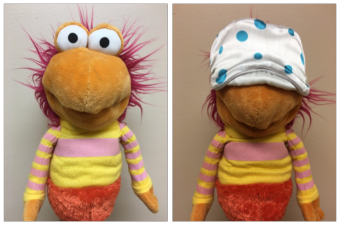
\includegraphics{figs/jazzy-1.pdf}
\caption{\label{fig:jazzy}The puppet, Jazzy, with and without the sleeping
mask.}
\end{figure}

\paragraph{Participants and
Procedure}\label{participants-and-procedure-1}

We recruited 42 English speaking children from the Bing Nursery School
at Stanford University. Children were between 3;1 and 5;2 years old
(Mean = 4;3). The experiment was carried out in a quiet room and all
sessions were videotaped. There was a small table and two chairs in the
room. Children sat on one side of the table and the experimenter and the
puppet on the other side facing the child. The groups of circles, small
stars, and big stars were placed in front of the child from left to
right. A deck of six cards was in front of the experimenter. As in study
1 with adults, the children went through three phases: introduction,
instruction, and test.

The goal of the introduction was for the experimenter to show the cards
to the children and make sure they recognized the animals and knew their
names. The experimenter showed the cards to the children and asked them
to label each animal. All children recognized the animals and could
label them correctly. In the instruction phase, children went through
three example trials. The experimenter explained that he was going to
play with the puppet first, so that the child could learn the game. He
removed the six introduction cards and placed a deck of three cards
face-down on the table. From top to bottom (first to last), the cards
had the following images: cat, elephant, cat and dog (Table
\ref{tab:instruction}). He put the sleeping mask on the puppet's eyes
and explained that the puppet is going to guess what animal is on the
cards. He then picked the first card and asked the puppet: \enquote{What
do you think is on this card?} The puppet replied with \enquote{There is
a dog}. The experimenter showed the cat-card to the child and explained
that when the puppet is \enquote{not right} he gets a circle. The pilot
study had shown that some children struggle with understanding the word
\enquote{wrong}, so \enquote{not right} was used instead. He then asked
the child to give the puppet a circle. Rewards were collected by the
experimenter and placed under the table to not distract the child. The
second trial followed the same pattern except that the puppet guessed
\enquote{right} and the experimenter invited the child to give the
puppet a big star. In the final trial, the puppet guessed that there is
a cat on the card when the card had a cat and a dog on it. The
experimenter said that the puppet was \enquote{a little right} and asked
the child to give him a little star.

\begin{longtable}[]{@{}lll@{}}
\caption{\label{tab:instruction} Instruction Trials.}\tabularnewline
\toprule
Card & Guess & Reward\tabularnewline
\midrule
\endfirsthead
\toprule
Card & Guess & Reward\tabularnewline
\midrule
\endhead
CAT & There is a dog! & Circle\tabularnewline
ELEPHANT & There is an elephant! & Big Star\tabularnewline
CAT-DOG & There is a dog! & Little Star\tabularnewline
\bottomrule
\end{longtable}

In the test phase, the experimenter removed the three instruction cards
and placed a deck of 16 randomized cards on the table. He explained that
it was the child's turn to play with the puppet. For each card, the
puppet provided a guess and the child provided the puppet with a reward.

\paragraph{Offline Annotations}\label{feedbackCoding}

While playing the game, children often provided spontaneous verbal
reactions to the puppet's guesses. During the analysis of the videos,
these verbal responses were categorized into four types: 1. None, 2.
Judgments, 3. Descriptions, and 4. Corrections. The first category
referred to cases where children did not say anything and only rewarded
the puppet. Judgments referred to linguistic feedback such as
\enquote{you are right!}, \enquote{yes}, \enquote{nope}, or \enquote{you
winned}. Such feedback only expressed judgments and complemented the
rewards. Descriptions were cases that the child simply mentioned what
was on the card: \enquote{cat!}, \enquote{dog and elephant!},
\enquote{There is a cat and a dog!} etc. Finally, corrections referred
to feedback that provided \enquote{focus words} (e.g. \emph{just},
\emph{only}, \emph{AND}) that acted like corrections to what the puppet
had said. Examples include: \enquote{Just a cat!}, \enquote{Both!},
\enquote{The two are!}, \enquote{Only cat!}, \enquote{cat AND dog} (with
emphasis placed on \emph{and}). In trials where the child provided both
judgments as well as descriptions or corrections (e.g. \enquote{Yes!
Cat!}), we placed the feedback into the more informative categories,
namely description or correction.

\subsubsection{Results}\label{results-1}

\begin{figure}
\centering
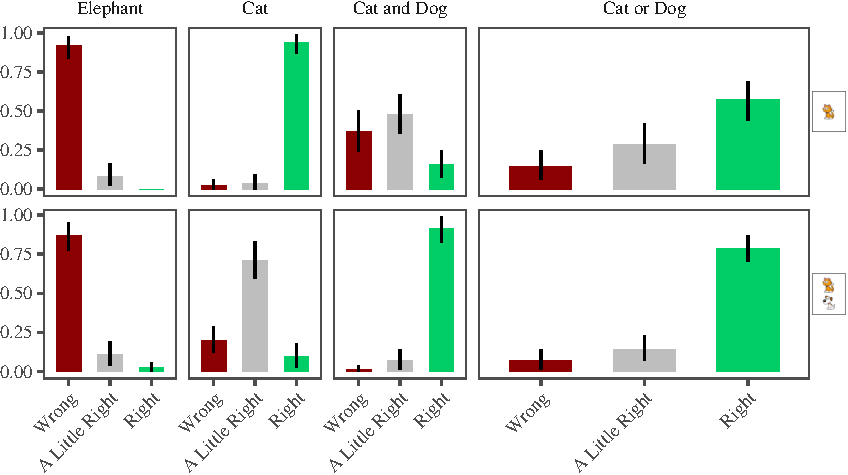
\includegraphics{figs/childrenTernaryPlot-1.pdf}
\caption{\label{fig:childrenTernaryPlot}Children's 3AFC judgments in the
connective guessing game.}
\end{figure}

Figure \ref{fig:childrenTernaryPlot} shows the results for children's
3AFC judgments. Starting from the left column, if the mentioned animal
was not on the card (e.g.~elephant), children judged the guess as
\enquote{wrong}. If the animal mentioned (e.g.~cat) was the only animal
on the card, children judged the guess to be \enquote{right}. Here we
ignore the results for trial types in which the animal mentioned was one
of the animals on the card. The reason is that such trials were used in
the instruction phase to introduce the \enquote{little bit right}
option, and the results are probably biased by the instructions.

In conjunctive guesses (e.g. \emph{cat and dog}), when only one of the
animals mentioned was on the card, children judged the guess as
\enquote{wrong} or \enquote{a little bit right}. However, if both
animals were on the card, they judged it \enquote{right}. In disjunctive
guesses (e.g. \emph{cat or dog}), when only one of the animals mentioned
was on the card, children considered the guess \enquote{right} or
\enquote{kinda right}. If both animals were on the card, it was
considered \enquote{right}. Figure \ref{fig:childAdultComp} compares the
results for children and adults' 3AFC judgments in the conjunction and
disjunction trials. The major difference between adults and children's
responses was disjunctive trials with two animals on the card. Most
children considered such trials as \enquote{right} while most adults
considered them as \enquote{kinda right}. In the next section, we use
Bayesian regression modeling to compare adults' and children's
three-alternative responses more systematically.

\begin{figure}
\centering
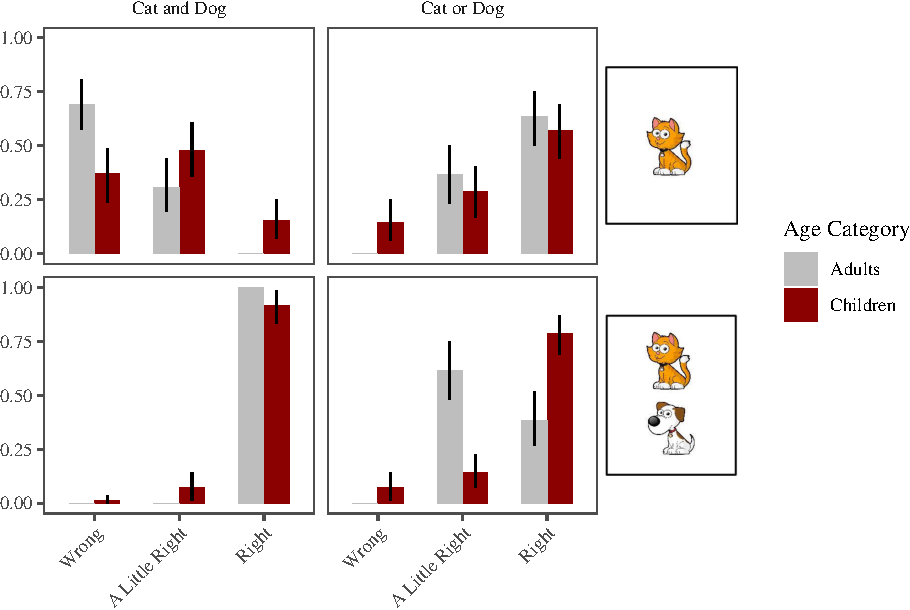
\includegraphics{figs/childAdultComp-1.pdf}
\caption{\label{fig:childAdultComp}Comparison of Adults' and Children's 3AFC
judgments.}
\end{figure}

\paragraph{Analysis and Statistical
Modeling}\label{analysis-and-statistical-modeling}

\begin{figure}
\centering
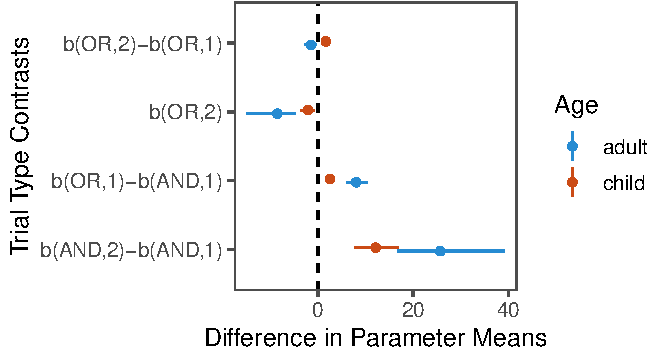
\includegraphics{figs/stanModelPlot-1.pdf}
\caption{\label{fig:stanModelPlot}Coefficients capturing the relevant
comparisons across conditions in 3AFC judgments in Study 1 and 2. In
naming the coefficients like b(OR,2), OR/AND represents the connective
used and the number 1/2 represents the number of animals on the card.
Error bars represent 99\% regions of highest posterior density.}
\end{figure}

We used the R package RStan for Bayesian statistical modeling to fit
separate ordinal mixed-effects logistic models for adults' and
children's judgments. The response variable had three ordered levels:
\emph{wrong}, \emph{kinda right}, and \emph{right}. The trial types
\emph{One-Animal-OR}, \emph{Two-Animals-OR}, \emph{One-Animal-AND}
constituted the (dummy-coded) fixed effects of the model with
\emph{Two-Animals-AND} set as the intercept. The model also included
by-subject random intercepts. The priors over trial types and the random
intercepts were set to \(\mathcal{N}(0,10)\). We also included
parameters \(C_1\) and \(C_2\), the two cutpoints delimiting the
logistic for 1) \emph{wrong} and \emph{kinda right} and 2) \emph{kinda
right} and \emph{right} responses, drawn with the prior
\(\mathcal{N}(0,1)\).\footnote{We used a tight prior in this case to
  decrease posterior correlations between cutpoints and intercept.} All
four chains converged after 3000 samples (with a burn-in period of 1500
samples).

We made inferences based on the highest-posterior density (HPD)
intervals for the coefficients estimated from each model. Because
predictors are dummy-coded, it's possible to examine contrasts of
interest by computing the difference between coefficients for pairs of
conditions we wish to contrast. In naming the coefficients like b(OR,2),
OR/AND represents the connective used and the number represents the
number of animals on the card. Figure \ref{fig:stanModelPlot} shows the
contrasts of interest: \emph{b(OR, 2)-b(OR,1)} represents the difference
between the estimated coefficients for the disjunction trials with two
animal on the card and those with only one; \emph{b(OR, 2)} represents
the difference between the estimated coefficients for the conjunction
trials with two animals and the disjunction trials with two animals; and
so on.

Overall, adults' and children's estimated coefficients are similar in
sign to one another, though adults' are more extreme. In the conjunction
trials (\emph{b(AND, 2)-b(AND,1)}), children and adults showed a strong
preference for the cards with two animals rather than one. At the same
time, given two animals on the card, children and adults showed a
preference for \emph{and} rather than \emph{or} (\emph{b(OR, 2)}).
However, with only one animal on the card, children and adults preferred
a disjunctive guess (\emph{b(OR, 1)-b(AND,1)}). These results are
compatible with the truth conditions of conjunction and disjunction.

The main difference between adults and children shows up in the contrast
between the disjunctive trial types: two animals vs.~only one
(\emph{b(OR, 2)-b(OR,1)}). On average, children rated disjunction trials
with two animals higher than those with only one. Adults on the other
hand showed the opposite pattern: they rated disjunction trials with two
animals lower. This pattern is compatible with current accounts of
pragmatic development that suggest children's interpretations tend to be
more literal than adults (Barner et al., 2011; Noveck, 2001; Papafragou
\& Musolino, 2003).

The slight preference children show for cards with two animals when the
guess is disjunctive (e.g. \enquote{cat or dog}) is also compatible with
the account proposed by Singh et al. (2016) and Tieu et al. (2016).
However, the effect seems much smaller here than was reported in their
studies. The comparison with conjunction trials makes it clear that
overall, children are not interpreting \emph{or} as a conjunction. The
effect in this study can be more accurately described as a preference in
truth value judgments for both disjuncts being true rather than a
conjunctive interpretation of disjunction. The results from children's
spontaneous linguistic feedback provide more evidence that children are
not interpreting \emph{or} as a conjunction. We will discuss these
results next.

\paragraph{Children's open-ended
feedback}\label{childrens-open-ended-feedback}

\begin{longtable}[]{@{}lll@{}}
\caption{\label{tab:feedbackCat} Definitions and Examples for the Feedback
Categories.}\tabularnewline
\toprule
\begin{minipage}[b]{0.15\columnwidth}\raggedright\strut
Category\strut
\end{minipage} & \begin{minipage}[b]{0.45\columnwidth}\raggedright\strut
Definition\strut
\end{minipage} & \begin{minipage}[b]{0.31\columnwidth}\raggedright\strut
Examples\strut
\end{minipage}\tabularnewline
\midrule
\endfirsthead
\toprule
\begin{minipage}[b]{0.15\columnwidth}\raggedright\strut
Category\strut
\end{minipage} & \begin{minipage}[b]{0.45\columnwidth}\raggedright\strut
Definition\strut
\end{minipage} & \begin{minipage}[b]{0.31\columnwidth}\raggedright\strut
Examples\strut
\end{minipage}\tabularnewline
\midrule
\endhead
\begin{minipage}[t]{0.15\columnwidth}\raggedright\strut
\textbf{None}\strut
\end{minipage} & \begin{minipage}[t]{0.45\columnwidth}\raggedright\strut
no verbal feedback\strut
\end{minipage} & \begin{minipage}[t]{0.31\columnwidth}\raggedright\strut
\strut
\end{minipage}\tabularnewline
\begin{minipage}[t]{0.15\columnwidth}\raggedright\strut
\textbf{Judgment}\strut
\end{minipage} & \begin{minipage}[t]{0.45\columnwidth}\raggedright\strut
provided verbal judgment mirroring the reward\strut
\end{minipage} & \begin{minipage}[t]{0.31\columnwidth}\raggedright\strut
\enquote{No!}, \enquote{Yes!} , \enquote{You are right!}\strut
\end{minipage}\tabularnewline
\begin{minipage}[t]{0.15\columnwidth}\raggedright\strut
\textbf{Description}\strut
\end{minipage} & \begin{minipage}[t]{0.45\columnwidth}\raggedright\strut
mentioned the animal(s) on the card\strut
\end{minipage} & \begin{minipage}[t]{0.31\columnwidth}\raggedright\strut
\enquote{elephant}, \enquote{cat and dog}\strut
\end{minipage}\tabularnewline
\begin{minipage}[t]{0.15\columnwidth}\raggedright\strut
\textbf{Correction}\strut
\end{minipage} & \begin{minipage}[t]{0.45\columnwidth}\raggedright\strut
used focus particles like \emph{only}/\emph{just}, emphasized \emph{and}
or used \emph{both}\strut
\end{minipage} & \begin{minipage}[t]{0.31\columnwidth}\raggedright\strut
\enquote{only cat}, \enquote{just elephant}, \enquote{both!},
\enquote{cat AND dog!}\strut
\end{minipage}\tabularnewline
\bottomrule
\end{longtable}

As explained in section \ref{feedbackCoding}, we also categorized and
annotated children's spontaneous and free-form verbal reactions to the
puppet's guesses. Table \ref{tab:feedbackCat} summarizes the definitions
and examples for each category and Figure \ref{fig:feedbackData} shows
the results. We should point out that each trial type had a similar
number of \enquote{None} cases. Some children remained more or less
silent throughout the experiment and only provided rewards to the
puppet. In the next study we ask children to provide feedback explicitly
and therefore we have no \enquote{None} responses. In the discussion and
analysis here we will not comment further on the \enquote{None} category
but focus on the other three categories.

\begin{figure}
\centering
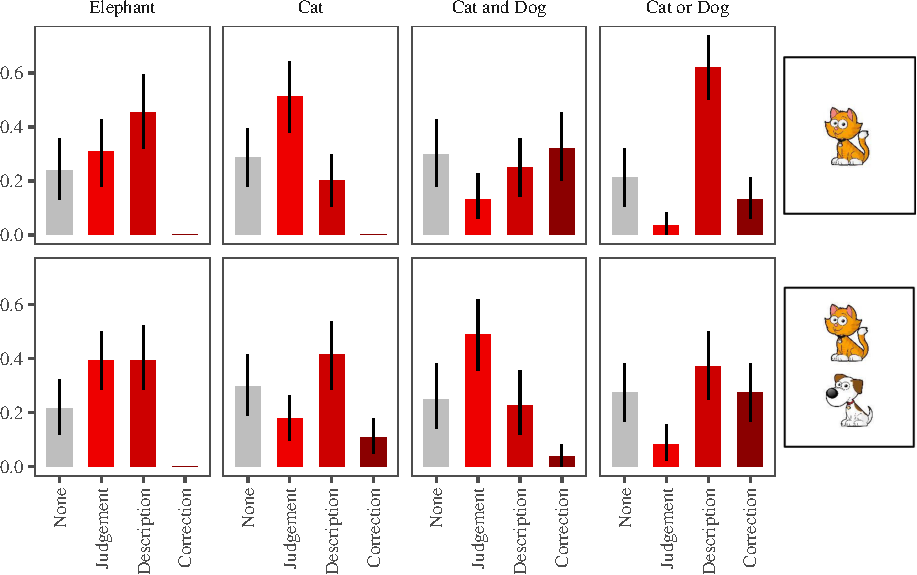
\includegraphics{figs/feedbackData-1.pdf}
\caption{\label{fig:feedbackData}Children's open-ended Feedback. Error bars
represent 95\% confidence intervals.}
\end{figure}

In the leftmost column, when the guessed animal was not on the card
(e.g. \enquote{there is an elephant}), children either provided
judgments like \enquote{No!} or described what was on the card (e.g.
\enquote{cat} or \enquote{cat and dog}). However, when the guessed
animal was the only animal on the card (e.g. \enquote{there is a cat}),
most children provided a positive judgment like \enquote{Yes}. When the
animal guessed was only one of the animals on the card, children
described what was on the card (e.g.~cat and dog).

In the critical trial types with conjunction and disjunction, children
showed a high rate of corrections and descriptions when there was only
one animal on the card (e.g.~cat) and the guess was a conjunction (e.g.
\enquote{there is a cat and a dog}). In their corrections, children used
the focus particles \emph{just} and \emph{only} as in \enquote{just a
cat} or \enquote{only a cat}. However, when both animals were on the
card and a conjunction was used (e.g. \enquote{there is a cat and a
dog}), children predominantly provided positive judgments like
\enquote{Yes!} and \enquote{You are right}. Considering disjunctive
guesses like \enquote{cat or dog}, when only one of the animals was on
the card, most children simply described what was on the card (e.g.
\enquote{cat}). However, when both animals were on the card, children
corrected the puppet by saying \enquote{Both!} or emphasizing \emph{and}
as in \enquote{cat AND dog!}.

We performed chi-squared goodness-of-fit tests to compare the feedback
distributions in the critical conditions with \emph{and} and \emph{or}.
Here we focus on those trials (the four bar charts on the right of
Figure \ref{fig:feedbackData}). Children's linguistic feedback showed
three patterns. First, the one-animal conjunctive and two-animal
disjunctive (top left and bottom right) trials contained a higher
proportion of corrections than the other trial types. These were trials
where the guesses were either false or infelicitous. In the conjunction
trials, a comparison of the feedback distribution in one-animal and
two-animal conditions was statistically significant (\(\chi^2\)(3, 83) =
201.65, p \textless{} .0001), suggesting that children gave different
feedback to true and false guesses. A similar numerical trend was
present in the disjunction trials, but it was not significant
(\(\chi^2\)(9, 4) = 12, p = 0.21).

Second, the one-animal disjunctive trials (top right) showed the highest
proportion of \enquote{descriptions}. These are trials in which the
guess is correct but not specific enough: it leaves two possibilities
open. These trials were significantly different from the one-animal
trials for conjunction (\(\chi^2\)(3, 83) = 62.16, p \textless{} .0001).
Finally, the two-animal conjunctive trials (bottom left) showed the
highest proportion of \enquote{judgments} such as \emph{You are right!}.
This was not surprising given that these trials represented the optimal
guessing scenario. These trials had a significantly different feedback
distribution from the matching disjunction trials (\(\chi^2\)(3, 84) =
184.98, p \textless{} .0001).

\subsubsection{Discussion}\label{discussion-1}

In study 2, we used a 3AFC judgment task to test children's
comprehension of logical connectives \emph{and} and \emph{or}. We
compared these results to those found in the 3AFC judgment task of study
1 with adults. The general comparison showed that adults and children
had similar patterns of judgments, except when both disjuncts were true.
In such cases, adults judged the disjunctive guess as not completely
right while most children judged it as completely right. There was even
a slight preference among children to rewarded the puppet more in such
cases, compared to cases of disjunction when only one disjunct was true.

To consider another measure of children's comprehension, we also looked
at children's spontaneous open-ended verbal feedback to the puppet's
guesses. Our analyses suggested that children recognized false and
infelicitous utterances with the connectives and provided appropriate
corrective feedback. As expected from an adult-like understanding of
connectives, children corrected the puppet most often when there was
only one animal on the card and the guess was conjunctive, or when there
were two animals on the card and the guess was disjunctive. Perhaps the
most important finding was that children increased their corrective
feedback in disjunctive guesses where both disjuncts were true, compared
to those with only one true disjunct. These findings differ from the
results of the 3AFC judgment task which suggested that children did not
find any infelicity with disjunctive guesses when both disjuncts were
true.

The analysis of children's open-ended feedback raises two important
issues. First, it runs counter to what the 3AFC judgment task suggests
with respect to exclusivity implicatures. The forced-choice task
suggests that children find such underinformative utterances as
unproblematic while analysis of their spontaneous feedback shows that
they provided more corrections to such utterances. Second, one of the
explanations for why children fail to derive implicatures is that they
cannot access the stronger alternative to the disjunction word
\emph{or}, namely \emph{and} (Barner et al., 2011). However, in the
context of the guessing game, some children explicitly mentioned the
word \emph{and}, as the word the puppet should have said instead of
\emph{or}. Interestingly, these children continued to reward the puppet
and considered the guess \enquote{right}, even though they corrected
him. This raises the possibility that forced-choice truth value
judgments underestimate children's pragmatic knowledge. In study 3, we
used both a 2AFC truth judgment task and an analysis of children's
open-ended feedback. If the findings of study 2 were on the right track,
we expected to replicate the same pattern in study 3, and find that
children's open-ended feedback better reflects their sensitivity to
pragmatic violations than the results of the 2AFC judgments.

\subsection{Study 3: Children's 2AFC judgments and open-ended
feedback}\label{study3}

This study used the same paradigm as study 2 but focused on children's
open-ended feedback and aimed at replicating the findings in study 2.
The main hypothesis was that four-year-olds provide corrective feedback
to the puppet if both disjuncts are true, but they do not consider this
infelicity to be grave enough to render the guess itself \enquote{wrong}
in a 2AFC judgment task. The main hypothesis along with relevant
analyses and predictions were preregistered in an \enquote{As Predicted}
format\footnote{The As Predicted PDF document is accessible at
  \url{https://aspredicted.org/x9ez2.pdf}.}.

\subsubsection{Methods}\label{methods-2}

\begin{longtable}[]{@{}lllll@{}}
\caption{\label{tab:study3info} Summary of Study 3 Methods}\tabularnewline
\toprule
\begin{minipage}[b]{0.19\columnwidth}\raggedright\strut
Study\strut
\end{minipage} & \begin{minipage}[b]{0.02\columnwidth}\raggedright\strut
N\strut
\end{minipage} & \begin{minipage}[b]{0.20\columnwidth}\raggedright\strut
Age\strut
\end{minipage} & \begin{minipage}[b]{0.11\columnwidth}\raggedright\strut
Mode\strut
\end{minipage} & \begin{minipage}[b]{0.32\columnwidth}\raggedright\strut
Response Options\strut
\end{minipage}\tabularnewline
\midrule
\endfirsthead
\toprule
\begin{minipage}[b]{0.19\columnwidth}\raggedright\strut
Study\strut
\end{minipage} & \begin{minipage}[b]{0.02\columnwidth}\raggedright\strut
N\strut
\end{minipage} & \begin{minipage}[b]{0.20\columnwidth}\raggedright\strut
Age\strut
\end{minipage} & \begin{minipage}[b]{0.11\columnwidth}\raggedright\strut
Mode\strut
\end{minipage} & \begin{minipage}[b]{0.32\columnwidth}\raggedright\strut
Response Options\strut
\end{minipage}\tabularnewline
\midrule
\endhead
\begin{minipage}[t]{0.19\columnwidth}\raggedright\strut
Study 3\strut
\end{minipage} & \begin{minipage}[t]{0.02\columnwidth}\raggedright\strut
50\strut
\end{minipage} & \begin{minipage}[t]{0.20\columnwidth}\raggedright\strut
3;6-5;9 (M = 4;7)\strut
\end{minipage} & \begin{minipage}[t]{0.11\columnwidth}\raggedright\strut
Study Room\strut
\end{minipage} & \begin{minipage}[t]{0.32\columnwidth}\raggedright\strut
Yes (Right)/No (Wrong) - Open-ended Feedback\strut
\end{minipage}\tabularnewline
\bottomrule
\end{longtable}

\paragraph{Materials and Design}\label{materials-and-design-2}

Study 3 was similar to Study 2 but differed in how children provided
their judgments. Based on the findings in Study 2, we focused on verbal
feedback, instead of rewards. We used two different ways of measuring
children's judgments. First, we encouraged children to provide verbal
feedback to the puppet. They were asked to say \enquote{yes} when the
puppet was right, \enquote{no} when he was not, and then help him say it
better. After children were done with this initial open-ended feedback,
for each trial we asked a forced choice yes/no judgment question:
\enquote{Was Jazzy (the puppet) right?}. This question elicited a 2AFC
response for each trial independent of children's earlier open-ended
response. These two measures allowed us to compare open-ended and binary
forced-choice judgments in the same setup.

\paragraph{Participants and
Procedure}\label{participants-and-procedure-2}

We recruited 50 English speaking children from the Bing Nursery School
at Stanford University. Children were between 3;6 and 5;9 years old
(Mean = 4;7). The setup and procedure were similar to Study 2, except
there were no rewards on the table. As before, participants sat through
three phases: introduction, instruction, and test. The introduction
phase made sure children knew the names of the animals on the cards. In
the instruction phase, they received four training trials, as shown in
Table \ref{tab:instructionStudy3}.

As in Study 2, the experimenter put a sleeping mask over the puppet's
eyes and explained that Jazzy (the puppet) was going to guess what
animal was on the cards. He then picked the first card and asked the
puppet: \enquote{What do you think is on this card?} The puppet replied
with \enquote{There is a dog}. The experimenter showed the cat-card to
the child and said: when Jazzy is \enquote{not right}, tell him
\enquote{no}. He then asked the child to say \enquote{no} to the puppet.
The second trial followed the same pattern except that the puppet
guessed \enquote{right} and the experimenter invited the child to say
\enquote{yes} to the puppet. There were two more instruction trials
before the test phase began. The test phase contained 16 randomized
trials, half of which contained guesses with the words \emph{and} and
\emph{or}. The randomization code as well as the details of the methods
are available on this paper's online repository.

\begin{longtable}[]{@{}lll@{}}
\caption{\label{tab:instructionStudy3} Instruction Trials for Study
3.}\tabularnewline
\toprule
Card & Guess & Response\tabularnewline
\midrule
\endfirsthead
\toprule
Card & Guess & Response\tabularnewline
\midrule
\endhead
CAT & there is a dog! & No!\tabularnewline
ELEPHANT & there is an elephant! & Yes!\tabularnewline
DOG-ELEPHANT & there is a cat! & No!\tabularnewline
DOG & there is a dog! & Yes!\tabularnewline
\bottomrule
\end{longtable}

\subsubsection{Results}\label{results-2}

We first look at the results of the 2AFC judgement task for each trial
type and compare them to those of the adults' in Study 1. Then we
analyze children's open-ended responses and compare them to the forced
choice responses obtained in the same trial types. For the 2AFC
judgments we excluded 26 trials (out of total 800) where children either
did not provide a Yes/No response or provided both (i.e. \enquote{Yes
and No}). The exclusions were almost equally distributed among different
types of guesses and cards. In the analysis of children's open-ended
feedback, we excluded 8 trials (out of total 800) where children either
did not provide any feedback or their feedback could not be categorized
into the existing categories.

\paragraph{Two-Alternative Forced Choice
Judgments}\label{two-alternative-forced-choice-judgments}

\begin{figure}
\centering
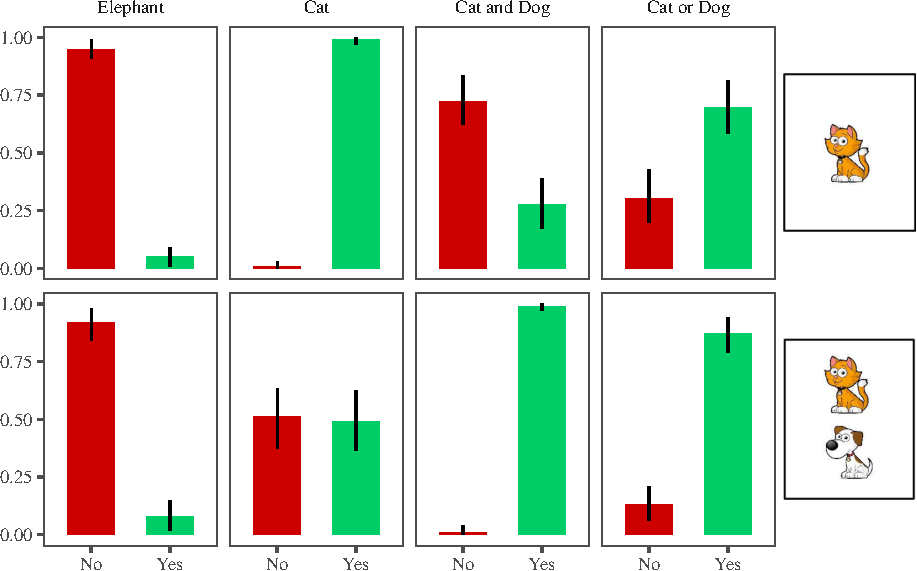
\includegraphics{figs/Study3tvjtPlot-1.pdf}
\caption{\label{fig:Study3tvjtPlot}Children's binary truth value judgments.}
\end{figure}

Figure \ref{fig:Study3tvjtPlot} shows children's 2AFC judgments. In the
leftmost column, when the animal guessed was not on the card
(e.g.~elephant), children considered the guess \enquote{wrong}. When the
animal guessed was the only animal on the card (e.g.~cat), children
considered the guess \enquote{right}. However, if the animal guessed
(e.g.~cat) was only one of the animals on the card, children were
equally split between \enquote{wrong} and \enquote{right} judgments. On
the other hand, almost all adults considered such guesses
\enquote{right} in their 2AFC judgments (Figure
\ref{fig:binaryAdultsPlot}). In such trial types, children seem to
interpret the guess \enquote{there is a cat} as \enquote{there is
\textbf{only} a cat}, while adults do not. This difference between
children and adults is unexpected for a theory of meaning acquisition
that assumes children are overall more logical or literal as
interpreters than adults (Noveck, 2001).

In the trials with \emph{and} and \emph{or}, children's judgments were
similar to those of adults. Figure \ref{fig:BinaryPlotComp} compares
adults' and children's 2AFC judgments. In trials with conjunction, when
only one of the animals was on the card, most children considered the
guess \enquote{wrong}. This is similar to adults' judgments, but
different in extent: adults were more consistent and unanimous in
rejecting such guesses. A mixed effects logistic regression with the
fixed effect of age category (adult vs.~child) and random effect of
subject found no significant difference between adults' and children's
responses in such trials (see Table \ref{tab:statsStudy3}, Conjunction -
One Animal).

\begin{longtable}[]{@{}lcccc@{}}
\caption{\label{tab:statsStudy3} Mixed effects logistic models for
conjunction and disjunction trials when only one disjunct was true, in
2AFC judgments of adults and children, using \texttt{glmer} in R's lme4
package. Formula:
\(Response \sim Age Category + (1|Subject)\).}\tabularnewline
\toprule
Trial Data & Coefficient & Standard Error & Z-Value &
P-value\tabularnewline
\midrule
\endfirsthead
\toprule
Trial Data & Coefficient & Standard Error & Z-Value &
P-value\tabularnewline
\midrule
\endhead
Conjunction - One Animal & -2.05 & 2.86 & -0.72 & 0.47\tabularnewline
Disjunction - One Animal & 1.34 & 1.79 & 0.75 & 0.45\tabularnewline
\bottomrule
\end{longtable}

In conjunctive guesses where both animals were on the card, both
children and adults were unanimous in considering the guess
\enquote{right}. In disjunctive trials when only one of the animals was
on the card, most children considered the guess \enquote{right}. This is
again similar to adults but differs from them in extent: adults more
consistently and unanimously judged such guesses as \enquote{right}. Yet
again, a mixed effects logistic regression with the fixed effect of age
(adult vs.~child) and random effect of subject found no significant
difference between adults' and children's responses in such trials (see
Table \ref{tab:statsStudy3}, Disjunction - One Animal). Adults and
children showed almost identical patterns of judgments in trials where
there was two animals on the card and the guess used the connective
\emph{or}. Children and adults did not differ in their rate of rejecting
disjunctive guesses when both disjuncts were true.

\begin{figure}
\centering
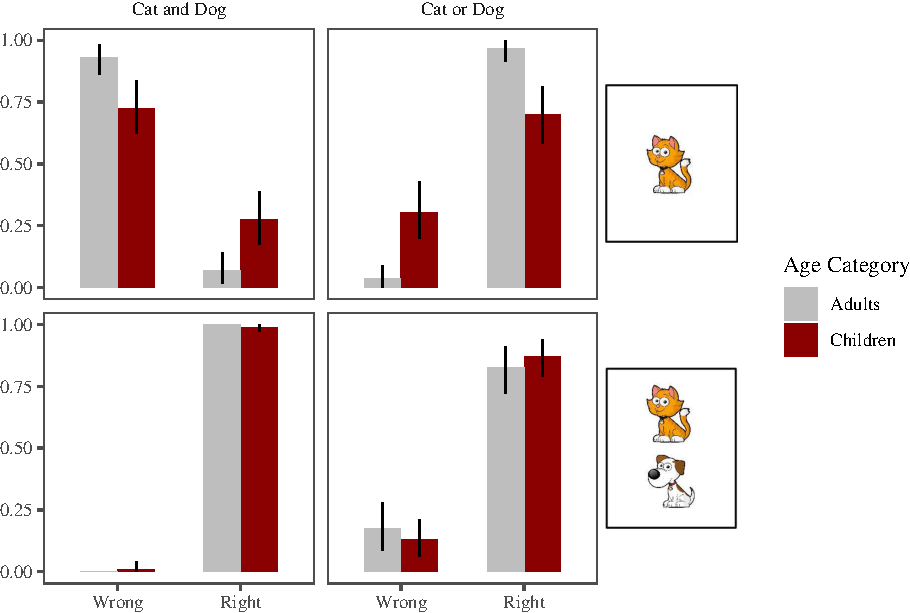
\includegraphics{figs/BinaryPlotComp-1.pdf}
\caption{\label{fig:BinaryPlotComp}The comparison of the 2AFC judgment task
for conjunction and disjunction trials in adults (study 1) and children
(study 3).}
\end{figure}

Finally, there is a small but significant preference in children's
judgments of disjunctive statements for both disjuncts to be true.
Comparing the disjunctive trials with one animal and two animals on the
card, a mixed-effects logistic model with the fixed effect of
disjunction type and the random effect of subjects found that children
had a slight preference for both animals to be on the card (\(b\)= 1.85,
\(se\)= 0.56, \(z\)= 3.32, \(p < 0.001\) ). There was a similar small
trend in children's three-alternative judgments in study 2. While this
was quite small compared to the other effects observed in these studies,
it nevertheless indicated a difference between children's and adults'
truth judgments. We return to this in more detail in section
\ref{conjunctive} of the General Discussion.

\paragraph{Open-ended Feedback}\label{open-ended-feedback}

\begin{figure}
\centering
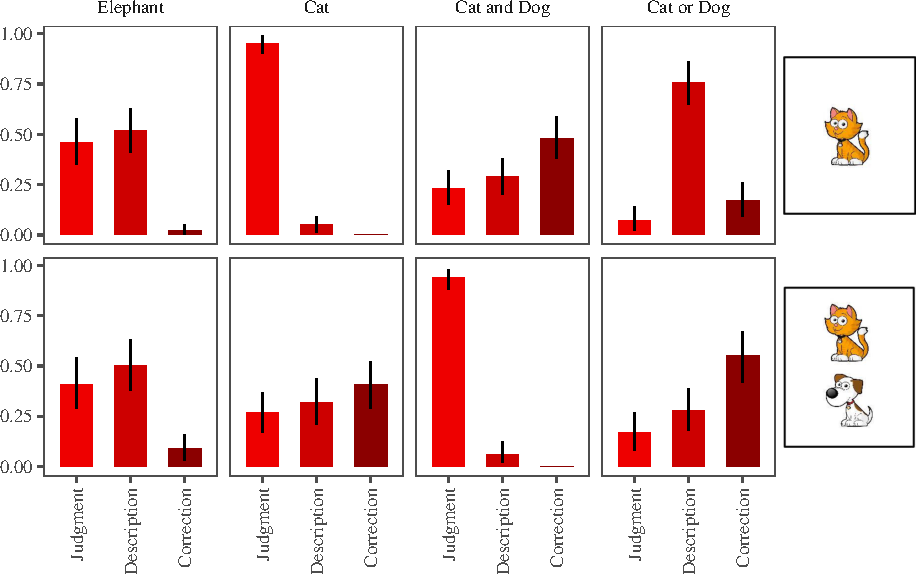
\includegraphics{figs/feedbackStudy3-1.pdf}
\caption{\label{fig:feedbackStudy3}Children's Open-ended Feedback in Study
3. Error bars represent 95\% confidence intervals.}
\end{figure}

Figure \ref{fig:feedbackStudy3} shows the distribution of children's
feedback to the puppet in Study 3 (see Table \ref{tab:feedbackCat} for
the definitions and examples of feedback categories). There were no
\enquote{None} responses in this study since the experimenter explicitly
asked children to provide feedback to the puppet. The distribution of
the responses in the other three categories (Judgment, Description, and
Correction) revealed a successful replication of Study 2.

Children's feedback showed four main patterns. First when the puppet
guessed an animal not on the card (e.g. \enquote{There is an
elephant!}), there is a split pattern between negative judgments like
\enquote{No!} and simply mentioning the animal on the card (e.g.
\enquote{Cat!}). Children provided no corrections on such trials, at
least the way we have defined them. Second, almost all children
responded with positive judgments like \enquote{Yes!} when the puppet's
guess accurately matched what was on the card. This was the case in
trials where there was only one animal on the card (e.g.~cat) and the
puppet mentioned it (e.g. \enquote{There is a cat!}), as well as trials
where there were two animals on the card and the puppet mentioned both
with a conjunction (e.g. \enquote{There is a cat and a dog!}). Third,
children provided the largest number of corrective feedback in trials
where the guess was either false or infelicitous. These included three
trial types: (a) the ones where there were two animals on the card
(e.g.~cat and dog) but the puppet only guessed one (e.g. \enquote{There
is a cat!}); (b) the ones where the puppet guessed two animals with
conjunction (e.g. \enquote{There is a cat and a dog!}) but only one of
them was on the card (e.g.~cat); and (c) the ones where there were two
animals on the card (e.g.~cat and dog), and the puppet guessed both but
used a disjunction (e.g. \enquote{There is a cat or a dog!}). Finally,
there was a pattern of feedback unique to disjunctive trials (e.g.
\enquote{There is a cat or a dog!}) with only one animal on the card
(e.g.~cat). In such cases, almost all children simply named the animal
on the card (e.g. \enquote{Cat!}).

\begin{figure}
\centering
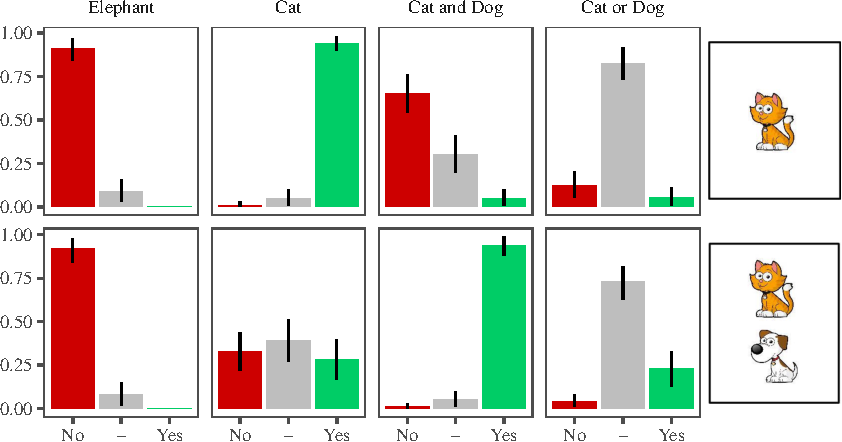
\includegraphics{figs/study3JudgmentPlot-1.pdf}
\caption{\label{fig:study3JudgmentPlot}Children's open-ended feedback to the
puppet's guesses. The x-axis shows whether children spontaneously
provided a yes (green), no (red), or other response (grey).}
\end{figure}

Figure \ref{fig:study3JudgmentPlot} breaks down children's open-ended
feedback based on whether children said \emph{Yes!}, \emph{No!}, or said
something else. Responses that were not yes/no judgments are grouped in
a middle category shown with a dash. The goal here is to compare
children's open-ended judgments with their forced choice judgments shown
in Figure \ref{fig:Study3tvjtPlot}. Children's open-ended judgments and
their forced choice judgments in study 3 show similar patterns for all
types of guesses except for disjunctive ones. In trials that the puppet
guessed a disjunction, the vast majority of children refused to provide
a yes/no judgment when they were not forced to. Instead, they described
the animal on the card or provided corrections to the puppet's
infelicitous disjunctive guess.

One way to interpret these results is that disjunctive guesses (with at
least one disjunct true) are considered neither right nor wrong. When
children were forced to provide wrong/right responses in the
experimental context, some conformed to the adult patterns of judgment
and some did not. However, it is possible that such deviations from
adult judgments do not reflect differences in the comprehension of
disjunction, but rather differences in how children map their
comprehension of disjunction onto the notions of \enquote{right} and
\enquote{wrong} when forced to do so.

\begin{figure}
\centering
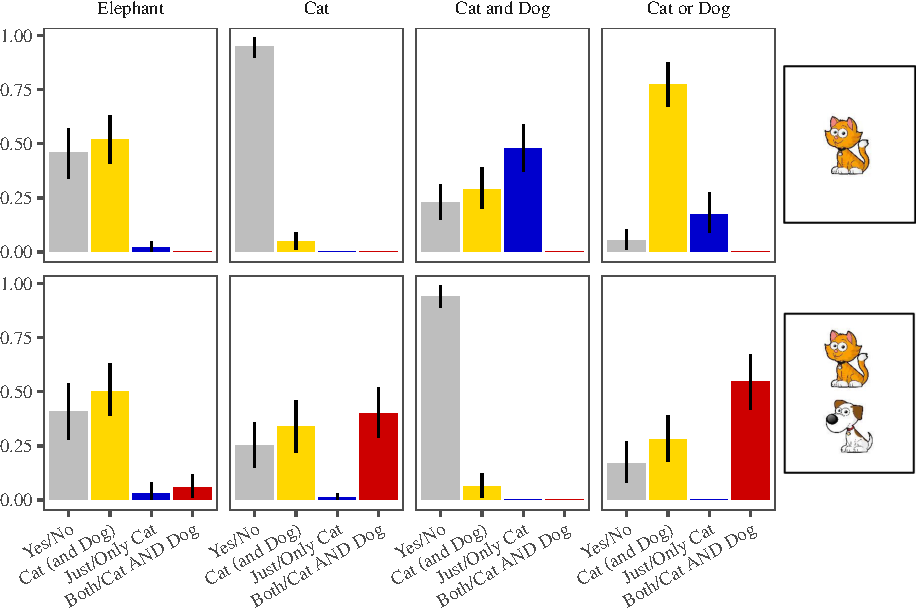
\includegraphics{figs/correctivePlot-1.pdf}
\caption{\label{fig:correctivePlot}Children's feedback categories in
disjunction trials.}
\end{figure}

Figure \ref{fig:correctivePlot} shows the proportion of feedback
categories other than yes/no judgments on the x-axis. Our goal here is
to display the trial types with corrective feedback (blue and red).
These trial types include: (1) conjunction when only one conjunct is
true (e.g.~guess: \enquote{There is a cat and a dog!}, card: cat), (2)
disjunction when both disjuncts are true (e.g.~guess: \enquote{There is
a cat or a dog}, card: cat and dog), and (3) simple guesses when two
animals were on the card (e.g. \enquote{There is a cat!}, card: cat and
dog). These trial types involved guesses that were either false or
infelicitous. Furthermore, the type of corrective feedback children
provided matched the type of mistakes made in the guesses. With
conjunctive guesses (e.g.~There is a cat and a dog!\enquote{) when there
was only one animal on the card (e.g.~cat), children provided exclusive
corrections (e.g.}Just/only a cat!\enquote{), suggesting that the other
animal (e.g.~dog) should have been excluded. When two animals were on
the card (e.g.~cat and dog) and the puppet used a disjunctive guess
(e.g.}There is a cat or a dog!\enquote{), or simple guess (e.g.}There is
a cat!``), children provided inclusive feedback, suggesting that another
animal should have been included. This is particularly notable in the
case of disjunction since both animals were mentioned, but children
still emphasized that the connective \emph{and} should have been used,
or that \emph{both} animals mentioned were on the card.

\subsubsection{Discussion}\label{discussion-2}

Study 3 measured children's comprehension of logical connectives in two
ways: First, with analyzing their open-ended feedback and second, with a
two-alternative forced choice task. First, we asked children to say
\emph{yes} to the puppet if he was right and \emph{no} if he was wrong.
However, children could provide any form of feedback they wanted.
Second, we followed children's open-ended feedback with a 2AFC question:
\enquote{Was the puppet right?} This way, we could measure children's
comprehension in two different ways in the same trial. Ideally, both
measures should show similar results. However, the findings were similar
for conjunctive guesses, but not disjunctive ones. Children avoided
binary right/wrong feedback with disjunction and preferred to provide
more nuanced feedback.

The 2AFC responses followed the predicted pattern: conjunctive guesses
were judged wrong if only one conjunct was true, and right if both were
true. Disjunctive guesses were judged right whether one or both
disjuncts were true. There was no significant difference in the 2AFC
task between the responses of children and those of adults in Study 1.
Children's open-ended feedback in Study 3 replicated the findings of
Study 2. Children provided more corrective feedback in false and
infelicitous trials than in true and felicitous ones. The corrective
feedback was tailored to the puppet's mistake. If the puppet used a
conjunction when there was only one animal on the card, children pointed
out that the other animal should have been excluded from the guess. They
used the exclusive adverbials \emph{just} and \emph{only} in their
feedback. If the puppet used a disjunction when both animals were on the
card, children stressed \emph{and} or \emph{both}, implying that both
animals should have been included.

While the 2AFC results suggested that children took no issue with
disjunctive guesses when both disjuncts were true, the analysis of their
corrective feedback showed that they provide appropriate corrections in
such cases and emphasized that the connective \emph{and} would have been
a better guess. Taking both measures together, we conclude that even
though children are aware of the problem with such guesses, they do not
consider them \emph{wrong}.

\subsection{General Discussion}\label{discussion}

We reported three studies on adults' and preschool children's
comprehension of the logical connectives \emph{and} and \emph{or}. The
first study used two- and three-alternative forced choice judgment tasks
with adults. In the 2AFC task, adult interpretations closely matched the
semantic accounts of \emph{and} and \emph{or} as conjunction and
inclusive disjunction. The 2AFC judgments did not register robust signs
of pragmatic infelicities. However, the 3AFC judgments showed signs of
pragmatic infelicities, especially in disjunctive guesses with true
disjuncts. When two animals where on the card (e.g.~cat and dog) and the
guess used \emph{or} (e.g. \emph{There is a cat or a dog!}),
participants were more likely to choose \enquote{kinda right} rather
than \enquote{right}.

The second study used a 3AFC judgment task with four-year-old children.
It also included an exploratory analysis of children's open-ended verbal
feedback to the puppet in the experimental setting. Children's
interpretations were similar to those of adults in the 3AFC task and
only differed for pragmatically infelicitous disjunctions. When both
disjuncts were true, adults tended to judge disjunctive guesses as
\enquote{kinda right}. This was evidence for the pragmatic infelicity of
such guesses. While, children judged such disjunctive statement as
\enquote{right}, the analysis of their open-ended feedback showed that
they took issue with such statements as well, and provided appropriate
corrective feedback.

In the third study, we focused on eliciting open-ended verbal feedback
from children and followed it with a 2AFC question. Children's 2AFC
responses reflected the semantics of the connectives \emph{and} and
\emph{or} as conjunction and inclusive disjunction. There was no
significant difference between children and adults in the 2AFC task.
Analysis of children's open-ended feedback replicated the findings in
study 2. Children provided more corrective feedback in false and
pragmatically infelicitous trials with the connectives than in
felicitous trials. The comparison of the 2AFC task and children's
open-ended responses showed that children are sensitive to the
infelicity of disjunctions with true disjuncts, even though they
consider them to be \enquote{right} guesses.

Previous studies had suggested that adults and preschool children differ
in their interpretation of disjunction in two ways. First, unlike
adults, children might interpret a disjunction as conjunction (Singh et
al., 2016; Tieu et al., 2016). Second, children might interpret
\emph{or} as inclusive disjunction when adults interpret it as exclusive
(Crain, 2012). The studies reported here provide evidence for the
hypothesis that these differences may be an artifact of the experimental
task and the type of measurement (Skordos et al. (2018), Katsos (2014)).

Considering the first difference, in the 2AFC and 3AFC judgment tasks we
found only small (but significant) preferences for both disjuncts being
true rather than only one. Combining the 2AFC and the verbal feedback
results, we expect that a child with strong conjunctive interpretation
of disjunction should have rejected a disjunctive guess when only one
disjunct was true, provided a \enquote{Just/Only} feedback, and accepted
the guess when both disjuncts were true without providing a correction.
We found no child in our sample that showed this pattern of responses.
Two children who consistently rejected a disjunction when only one
disjunct was true, provided corrective feedback when one or both
disjuncts were true. Therefore while it is possible that some children
interpret \emph{or} as \emph{and}, our results did not show a common or
consistent effect.

We would like to add that conjunctive interpretations of disjunction,
even when robustly observed, can have at least two potential
explanations. First, non-linguistic interpretive strategies and
preferences, due to task demands or unknown connective meaning (Clark,
1973; Paris, 1973), and second, pragmatic enrichment, common in
free-choice contexts (Singh et al., 2016; Tieu et al., 2016). As
explained in section \ref{litreview}, previous research provides
substantial evidence for task-related increase in conjunctive readings
of disjunction (Braine \& Rumain, 1981; Neimark \& Slotnick, 1970;
Paris, 1973; Skordos et al., 2018). In order to show instances of
pragmatically enriched conjunctive readings in preschool children, it is
important to first rule out task-related conjunctive interpretations.

Considering the second difference, namely the lower rate of exclusivity
inferences in preschool children, our studies provided evidence that the
choice of measurement may play an important role. In the 3AFC judgment
task when two animals were on the card (e.g.~card: cat and dog, guess:
\enquote{There is a cat or a dog}), adults were more likely to choose
\enquote{kinda right} than children were. Children mostly chose
\enquote{right}. However, in their free-form feedback, children
corrected such utterances and suggested that the connective \emph{and}
should have been used instead of \emph{or}.

There have been at least four major proposals to account for children's
perceived low rate of \enquote{implicature computation}: processing
difficulty (Pouscoulous, Noveck, Politzer, \& Bastide, 2007; Reinhart,
2004), non-adult-like lexical entry (Barner et al., 2011; Horowitz,
Schneider, \& Frank, 2017), pragmatic tolerance (Katsos \& Bishop,
2011), and the role of experimental measurement (Katsos, 2014). Below we
argue that the first three cannot explain the reported results of
children's forced judgments and free-form feedback, and that these
results highlight the role of experimental measurement as a source of
perceived differences in children and adults pragmatic inferences.

\textbf{1. Processing difficulty.} First, processing accounts locate the
problem in children's processing capacities such as working memory. They
suggest that pragmatic computations are cognitively taxing and children
lack the appropriate processing resources to carry them out
appropriately. A prediction of processing accounts (at least in their
current format) is that children will show reduced implicature
computations for all types of implicatures -- scalar or not. This
prediction was not borne out in our experimental results here. In Study
3, children were much more likely than adults to call a simple guess
(e.g. \emph{There is a cat!}) \enquote{wrong} if there were two animals
on the card (e.g.~cat and dog). In other words, children's
interpretations were much more exhaustive than adults. Processing
accounts do not predict that children may derive implicatures at a
higher rate than adults but this is what we found, at least for the
traditional interpretation of the judgment task.

\textbf{2. Non-adult-like Lexicon.} Several proposals blame the
structure of the child's lexicon for the alleged failure in deriving
implicatures. The assumption is that the child's lexical entry for
scalar items must include three elements for successful derivation: 1.
the semantics of the weak term (e.g. \emph{some}, \emph{or}) 2. the
semantics of the strong term (e.g. \emph{all},\emph{and}); and possibly
3. a scale that recognizes the stronger term as an alternative to the
weaker one (e.g. \textless{}\emph{some}, \emph{all}\textgreater{},
\textless{}\emph{or}, \emph{and}\textgreater{}). Each of these elements
have been pinpointed as the source of the problem in previous studies
(Barner et al., 2011; Horowitz et al., 2017; Katsos \& Bishop, 2011).
However none of them seem to apply to the results reported here.

If children in this study lack the semantics of the connective
\emph{or}, we would expect them to either perform at chance or default
to a conjunctive interpretation. Neither prediction was borne out in
studies 2 and 3. Furthermore, children's free-form linguistic feedback
in both studies suggested that children understood disjunction well
enough to provide relevant feedback. So this explanation seems unlikely.
The problem cannot be that children do not know the meaning of
\emph{and} either. Children's performance in both study 2 and 3 for
conjunction trials show that they understand its meaning very well.
Finally, comparing children's truth value judgments and their free-form
verbal feedback, we found that many children judged a disjunction with
true disjuncts as \enquote{right}, yet went on to correct the puppet and
explicitly mention \emph{and} as the connective he should have used. If
children could not access the stronger alternative, they could not have
mentioned it in their feedback either. And if accessing the stronger
alternative would have resulted in expressing sub-optimal judgments,
they should not have judged the guess as \enquote{right}.

\textbf{3. Pragmatic Tolerance.} Katsos \& Bishop (2011) suggested that
children tend to tolerate pragmatic infelicities more than adults. They
showed that when children were provided with a 2AFC judgment task, they
considered a description with the scalar term \emph{some} as
\enquote{right} when \emph{all} was more informative (e.g. \emph{The
turtle played with some of the balls.}, Scene: the turtle played with
all the balls.) However, when they are presented with three options
(small, big, and huge strawberries) in a 3AFC task, they choose the
middle option in the same type of trials. They argued that children
tolerate pragmatic infelicities and do not regard them as
\enquote{wrong}. As in a processing account, the tolerance account
predicts that scalar and ad-hoc implicatures will be similarly affected.
However, our results did not match those of Katsos \& Bishop (2011).
When children were presented with a 3AFC task, they chose the highest
reward (and not the middle option) for uses of \emph{or} when \emph{and}
was more informative. Second, and more importantly, we found different
patterns for exhaustive and scalar inferences as mentioned before. This
is not predicted by the tolerance account unless we assume that children
are more tolerant towards violations of scalar inferences than they are
towards exhaustive ones. While this is not currently assumed in the
literature, it is a possible adjustment. However, we would like address
this issue by focusing on another related factor: the role of
measurement in estimates of children's pragmatic capacity (Katsos,
2014).

\textbf{4. The Role of Measurment.} Two observations in the current
studies provide support for the hypothesis that methodological issues,
and more specifically issues of measurement contribute to the
differences found between adults and children in pragmatic capacity.
First, Study 1 showed that even for adults, the estimates of adult
infelicity rates may differ based on the number of alternatives in the
forced choice task. A 2AFC task underestimated adults' sensitivity to
pragmatic infelicity. In fact, in a follow up study, we systematically
varied the number of response options and replicated the results
presented here (see Jasbi, Waldon, and Degen in press). Second,
children's open-ended linguistic feedback in the experimental context
better reflected their sensitivity to pragmatic nuances than the
forced-choice judgment tasks. Third, children showed a higher rate of
\enquote{wrong} judgments for cases of exhaustive inferences (simple
guesses with two animals on the card) than adults did. While a
difference in sensitivity to ad-hoc vs.~scalar implicatures has been
reported and argued for before (Horowitz et al., 2017; Stiller, Goodman,
\& Frank, 2015), a higher sensitivity than adults is not predicted by
any of the current accounts.

\begin{figure}
\centering
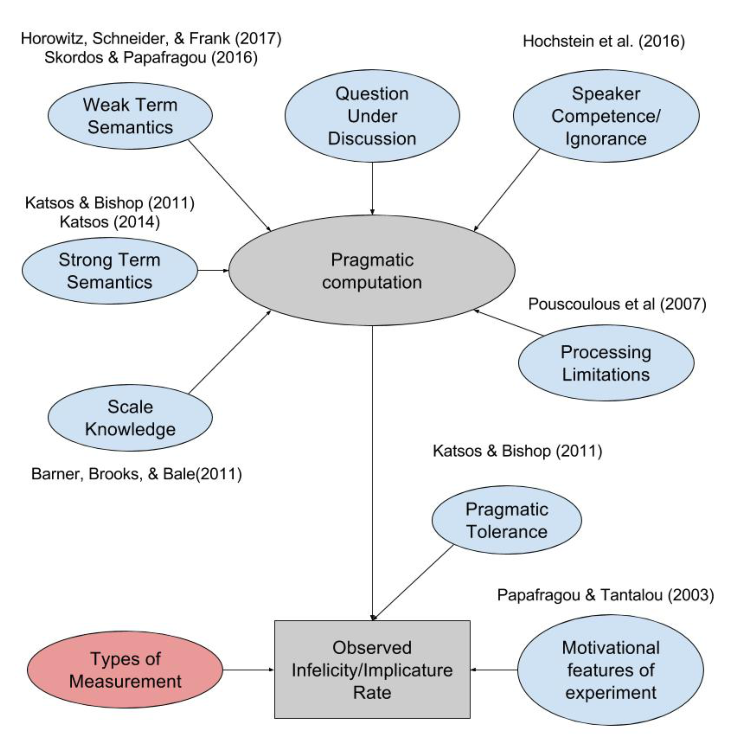
\includegraphics{figs/implicatureGraph-1.pdf}
\caption{\label{fig:implicatureGraph}Factors that could affect pragmatic
computations and the estimates of these computations in the experimental
settings}
\end{figure}

Figure \ref{fig:implicatureGraph} shows a summary of the factors that
are proposed to affect pragmatic computations. As Pouscoulous \& Noveck
(2009) and Katsos (2014) have suggested, the central issue is
\enquote{the rate} at which children and adults manifest pragmatic
reasoning in the experimental setting. No one doubts children's capacity
to perform such computations. At issue is the extent to which children
and adults compute specific implicatures. As Katsos (2014) pointed out,
it seems reasonable to assume that all these factors play some part
here. What matters is the degree to which each contributes to the
outcome.

The results of the studies reported here suggest that it is important to
distinguish between factors that affect pragmatic computations and those
that affect the observed \enquote{rate} in an experimental setting. As
we showed in Study 1, given the number of alternatives in the forced
choice task (2AFC vs.~3AFC), we may get different estimates of adults'
rate of infelicity judgments, but we cannot assume that there is a
difference in adults' pragmatic capacities in these two tasks. A similar
situation exists when we compare children's forced choice measures of
infelicity and their open-ended feedback.

In order to better understand the differences between adults and
children's semantic and pragmatic capacities, it is necessary to have a
good understanding of how our measurements affect estimates of adults
and children's performance in the experimental tasks. Children may be no
more capable of making exhaustive inferences than adults and no less
capable of making scalar inferences either. They may simply have a
different construal of the wrong-right scale and of what the
forced-choice task is about. The concepts \enquote{right} and
\enquote{wrong} are as much subject to developmental change and
differences between adults and children as are scalar items that
constitute the focus of our studies. Relying on a single type of
measurement increases the risk of measurement-specific conclusions.
Using multiple measurements in the same task can provide converging
evidence for felicity/infelicity or presence/absence of specific
inferences. Ultimately, in order to capture semantic and pragmatic
competences of adults and (especially) children, we need to develop
methods that can reliably tap into specific dimensions of meaning.

\subsection{Conclusion}\label{conclusion}

We provided three studies that tested adults and children's
comprehension of disjunction in existential sentences using three
different measures: binary forced-choice truth value judgments (2AFC
task), ternary forced-choice truth value judgments (3AFC task), and
free-form verbal feedback. The results showed that for each population,
different measures are sensitive to different aspects of meaning. The
binary measure captured children and adults intutions about truth values
well: it showed that they considered a disjunction as inclusive in
existential sentences of the guessing game. Ternary judgments provided
evidence for adults pragmatic inferences: adults often considered a
disjunction when both disjuncts were true as \enquote{kinda right} and
not completely right. For children, the ternary judgments did not
register such an effect, but their free-form verbal feedback did. When
both disjuncts were true, children verbally corrected the puppet and
suggested that he should have said \emph{and} instead of \emph{or}. The
combination of children's truth valued judgments and their verbal
feedback suggested that on average, children in our sample understood
that when both propositions are true, their conjunction and disjunction
are true yet conjunction makes a more appropriate and felicitous
utterance.

Since Tarski's original observations on disjunction, research in
semantics and pragmatics has shown that the variety of interpretations
Tarski observed are in fact distinct types of meaning observed in all
aspected of langauge and connected to distinct processes that generate
them. Therefore, while the inclusive interpretation is hypothesized to
be part of \emph{or}'s semantics, exclusivity and ignorance
interpretations are analyzed as distinct pragmatic inferences generated
separately. This theoretical insight has in turn lead developmental
researchers to seek distinct developmental mechanisms for each type of
meaning. The results of the studies reported here suggest that as more
and more varieties of meaning become subject of experimental study, we
also need to develop measures especially suited to capture the aspect of
meaning under investigation.

\newpage

\section{References}\label{references}

\setlength{\parindent}{-0.5in} \setlength{\leftskip}{0.5in}

\hypertarget{refs}{}
\hypertarget{ref-barner2011accessing}{}
Barner, D., Brooks, N., \& Bale, A. (2011). Accessing the unsaid: The
role of scalar alternatives in children's pragmatic inference.
\emph{Cognition}, \emph{118}(1), 84--93.

\hypertarget{ref-braine1981development}{}
Braine, M. D., \& Rumain, B. (1981). Development of comprehension of
``or'': Evidence for a sequence of competencies. \emph{Journal of
Experimental Child Psychology}, \emph{31}(1), 46--70.

\hypertarget{ref-chierchia1998some}{}
Chierchia, G., Crain, S., Guasti, M. T., \& Thornton, R. (1998).
``Some'' and ``or'': A study on the emergence of logical form. In
\emph{Proceedings of the Boston University conference on language
development} (Vol. 22, pp. 97--108). Somerville, MA: Cascadilla Press.

\hypertarget{ref-chierchia2001acquisition}{}
Chierchia, G., Crain, S., Guasti, M. T., Gualmini, A., \& Meroni, L.
(2001). The acquisition of disjunction: Evidence for a grammatical view
of scalar implicatures. In \emph{Proceedings of the 25th Boston
University conference on language development} (pp. 157--168).
Somerville, MA: Cascadilla Press.

\hypertarget{ref-chierchia2004semantic}{}
Chierchia, G., Guasti, M. T., Gualmini, A., Meroni, L., Crain, S., \&
Foppolo, F. (2004). Semantic and pragmatic competence in children's and
adults' comprehension of or. In I. Noveck \& D. Sperber (Eds.),
\emph{Experimental pragmatics} (pp. 283--300). Basingstoke: Palgrave
Macmillan.

\hypertarget{ref-clark1973non}{}
Clark, E. V. (1973). Non-linguistic strategies and the acquisition of
word meanings. \emph{Cognition}, \emph{2}(2), 161--182.

\hypertarget{ref-crain2012emergence}{}
Crain, S. (2012). \emph{The emergence of meaning}. Cambridge: Cambridge
University Press.

\hypertarget{ref-crain2008logic}{}
Crain, S., \& Khlentzos, D. (2008). Is logic innate?
\emph{Biolinguistics}, \emph{2}(1), 024--056.

\hypertarget{ref-crain2010logic}{}
Crain, S., \& Khlentzos, D. (2010). The logic instinct. \emph{Mind \&
Language}, \emph{25}(1), 30--65.

\hypertarget{ref-crain1998investigations}{}
Crain, S., \& Thornton, R. (1998). \emph{Investigations in universal
grammar: A guide to experiments on the acquisition of syntax and
semantics}. Cambridge, MA: MIT Press.

\hypertarget{ref-crain2000acquisition}{}
Crain, S., Gualmini, A., \& Meroni, L. (2000). The acquisition of
logical words. \emph{LOGOS and Language}, \emph{1}, 49--59.

\hypertarget{ref-goro2004acquisition}{}
Goro, T., \& Akiba, S. (2004). The acquisition of disjunction and
positive polarity in Japanese. In \emph{Proceedings of the 23rd West
Coast conference on formal linguistics} (pp. 251--264). Somerville, MA:
Cascadilla Press.

\hypertarget{ref-grice1975logic}{}
Grice, H. P. (1975). Logic and conversation. \emph{1975}, 41--58.

\hypertarget{ref-grice1989studies}{}
Grice, H. P. (1989). \emph{Studies in the way of words}. Cambridge, MA:
Harvard University Press.

\hypertarget{ref-gualminicrain2002}{}
Gualmini, A., \& Crain, S. (2002). Why no child or adult must learn de
Morgan's laws. In \emph{Proceedings of the Boston University conference
on language development}. Somerville, MA: Cascadilla Press.

\hypertarget{ref-gualmini2000}{}
Gualmini, A., Crain, S., \& Meroni, L. (2000). Acqisition of disjunction
in conditional sentences. In \emph{Proceedings of the boston university
conference on language development}.

\hypertarget{ref-horowitz2017trouble}{}
Horowitz, A. C., Schneider, R. M., \& Frank, M. C. (2017). The trouble
with quantifiers: Exploring children's deficits in scalar implicature.
\emph{Child Development}.

\hypertarget{ref-piaget1958growth}{}
Inhelder, B., \& Piaget, J. (1958). \emph{The growth of logical thinking
from childhood to adolescence: An essay on the construction of formal
operational structures} (Vol. 84). London: Routledge.

\hypertarget{ref-jasbiWaldonDegan2017}{}
Jasbi, M., Waldon, B., \& Degen, J. (submitted). \emph{Linking
hypothesis and number of response options modulate inferred scalar
implicature rate}.

\hypertarget{ref-johansson1975preschool}{}
Johansson, B. S., \& Sjolin, B. (1975). Preschool children's
understanding of the coordinators ``and'' and ``or''. \emph{Journal of
Experimental Child Psychology}, \emph{19}(2), 233--240.

\hypertarget{ref-katsos2014scalar}{}
Katsos, N. (2014). Scalar implicature. In D. Matthews (Ed.),
\emph{Pragmatic development in first language acquisition} (Vol. 10, p.
183---198). Amsterdam: John Benjamins.

\hypertarget{ref-katsos2011pragmatic}{}
Katsos, N., \& Bishop, D. V. (2011). Pragmatic tolerance: Implications
for the acquisition of informativeness and implicature.
\emph{Cognition}, \emph{120}(1), 67--81.

\hypertarget{ref-neimark1970}{}
Neimark, E. D. (1970). Development of comprehension of logical
connectives: Understanding of ``or''. \emph{Psychonomic Science},
\emph{21}(4), 217--219.

\hypertarget{ref-neimarkSlotnick1970}{}
Neimark, E. D., \& Slotnick, N. S. (1970). Development of the
understanding of logical connectives. \emph{Journal of Educational
Psychology}, \emph{61}(6p1), 451.

\hypertarget{ref-neisser1962hierarchies}{}
Neisser, U., \& Weene, P. (1962). Hierarchies in concept attainment.
\emph{Journal of Experimental Psychology}, \emph{64}(6), 640.

\hypertarget{ref-nitta1966basic}{}
Nitta, N., \& Nagano, S. (1966). Basic logical operations and their
verbal expressions: Child's conception of logical sum and product.
\emph{Research Bulletin of the National Institute for Educational
Research, Tokyo}, \emph{7}, 1--27.

\hypertarget{ref-notley2012notevery}{}
Notley, A., Thornton, R., \& Crain, S. (2012). English-speaking
children's interpretation of disjunction in the scope of ``not every''.
\emph{Biolinguistics}, \emph{6}(1), 32--69.

\hypertarget{ref-notley2012children}{}
Notley, A., Zhou, P., Jensen, B., \& Crain, S. (2012). Children's
interpretation of disjunction in the scope of ``before'': A comparison
of English and Mandarin. \emph{Journal of Child Language},
\emph{39}(03), 482--522.

\hypertarget{ref-noveck2001children}{}
Noveck, I. A. (2001). When children are more logical than adults:
Experimental investigations of scalar implicature. \emph{Cognition},
\emph{78}(2), 165--188.

\hypertarget{ref-papafragou2003scalar}{}
Papafragou, A., \& Musolino, J. (2003). Scalar implicatures: Experiments
at the semantics--pragmatics interface. \emph{Cognition}, \emph{86}(3),
253--282.

\hypertarget{ref-paris1973comprehension}{}
Paris, S. G. (1973). Comprehension of language connectives and
propositional logical relationships. \emph{Journal of Experimental Child
Psychology}, \emph{16}(2), 278--291.

\hypertarget{ref-pouscoulous2009going}{}
Pouscoulous, N., \& Noveck, I. A. (2009). Going beyond semantics: The
development of pragmatic enrichment. In S. Foster-Cohen (Ed.),
\emph{Language acquisition} (pp. 196--215). Berlin: Springer.

\hypertarget{ref-pouscoulous2007developmental}{}
Pouscoulous, N., Noveck, I. A., Politzer, G., \& Bastide, A. (2007). A
developmental investigation of processing costs in implicature
production. \emph{Language Acquisition}, \emph{14}(4), 347--375.

\hypertarget{ref-reinhart2004processing}{}
Reinhart, T. (2004). The processing cost of reference set computation:
Acquisition of stress shift and focus. \emph{Language Acquisition},
\emph{12}(2), 109--155.

\hypertarget{ref-Singh2016}{}
Singh, R., Wexler, K., Astle-Rahim, A., Kamawar, D., \& Fox, D. (2016).
Children interpret disjunction as conjunction: Consequences for theories
of implicature and child development. \emph{Natural Language Semantics},
\emph{24}(4), 305--352.

\hypertarget{ref-skordosEtal2018}{}
Skordos, D., Feiman, R., Bale, A., \& Barner, D. (2018, July). \emph{Do
children interpret ``or'' conjunctively?} Retrieved from
\url{https://osf.io/2srxk/}

\hypertarget{ref-stiller2015ad}{}
Stiller, A. J., Goodman, N. D., \& Frank, M. C. (2015). Ad-hoc
implicature in preschool children. \emph{Language Learning and
Development}, \emph{11}(2), 176--190.

\hypertarget{ref-strawson1950referring}{}
Strawson, P. F. (1950). On referring. \emph{Mind}, \emph{59}(235),
320--344.

\hypertarget{ref-su2014acquisition}{}
Su, Y. (2014). The acquisition of logical connectives in child Mandarin.
\emph{Language Acquisition}, \emph{21}(2), 119--155.

\hypertarget{ref-su2013disjunction}{}
Su, Y., \& Crain, S. (2013). Disjunction and universal quantification in
child mandarin. \emph{Language and Linguistics}, \emph{14}(3), 599--631.

\hypertarget{ref-suppes1969young}{}
Suppes, P., \& Feldman, S. (1969). \emph{Young children's comprehension
of logical connectives.} \emph{ERIC}. Department of Health, Education,
Welfare. Office of Education.

\hypertarget{ref-tarski1941logic}{}
Tarski, A. (1941). \emph{Introduction to logic and to the methodology of
the deductive sciences}. Oxford University Press.

\hypertarget{ref-tieu2016}{}
Tieu, L., Yatsushiro, K., Cremers, A., Romoli, J., Sauerland, U., \&
Chemla, E. (2016). On the role of alternatives in the acquisition of
simple and complex disjunctions in french and japanese. \emph{Journal of
Semantics}.






\end{document}
